\chapter{\label{ch:michel}Study of Michel Electron Reconstruction in \protodune{}}

\minitoc

\noindent
Studying electrons in the tens of MeV energy range can provide valuable input
into reconstruction techniques and energy uncertainty for astrophysical
neutrinos from supernova bursts. Understanding the response of LArTPC
detectors to electrons in this range will be important for any large scale
LArTPC experiment wishing to study supernova bursts. At these energies,
electron interactions have large contributions from both ionisation energy
loss and radiative energy loss and, therefore, they have a distinctive 
signature, which is neither track--like nor shower--like. As a result, 
low--energy electrons require dedicated reconstruction algorithms to maximise 
the overall reconstruction performance.

This chapter will discuss an approach to low--energy electron reconstruction
in LArTPC detectors, based on the use of convolutional neural networks and
semantic segmentation. Michel electron events from \protodune{} will be used
to test the performance of this technique, and to provide an estimate of the
energy uncertainty of LArTPC detectors for low--energy electrons.

In this Chapter, Section \ref{ME_LAr} will discuss the signature left by Michel
electrons in liquid argon, and the implications of this signature on
reconstructing Michel electron events in \protodune{}. This will be followed by
a discussion of the algorithm used to select Michel electron events in Section
\ref{ME_ES}. The Michel electron event reconstruction will be discussed in
Section \ref{ME_R}, along with a discussion of the reconstruction performance
and a comparison to the results of other LArTPC experiments. Finally, the
results presented in this chapter and their implications for the DUNE Far 
Detector will be summarised in Section \ref{ME_EU}.


\section{Michel Electrons in Liquid Argon} \label{ME_LAr}
Michel electrons are produced when a muon decays at rest. In vacuum, this
decay gives rise to a characteristic energy spectrum which has a sharp
cut--off at around 50 MeV, corresponding to half the muon mass. In matter, it
is also possible for $\mu^-$ to be captured on nuclei before they decay, this
causes a broadening of the Michel electron spectrum for these events. A
comparison of the Michel electron energy spectrum for free $\mu^\pm$ and
captured $\mu^-$ is given in Figure \ref{fig:michel_spec}. The capture process
occurs roughly 70\% of the time for negative muons in liquid argon, therefore,
in \protodune{}, the observed Michel electron energy spectrum is a combination
of the two processes in similar quantities.
\begin{figure}

	\centering
	\begin{subfigure}[b]{0.67\textwidth}
		\centering
		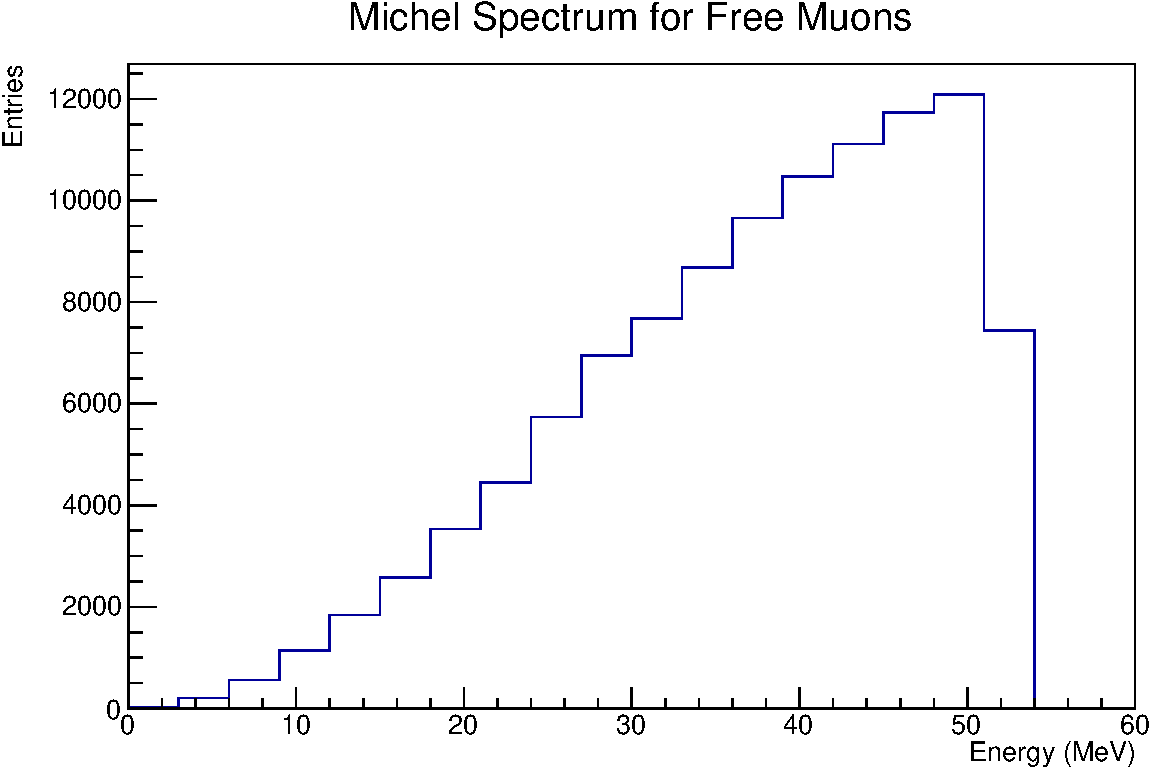
\includegraphics[width=\textwidth]{figures/michel_spec_free.pdf}
		\caption {Free Muons.}
		\label{fig:michel_spec_free}
	\end{subfigure}
	\begin{subfigure}[b]{0.67\textwidth}
		\centering
		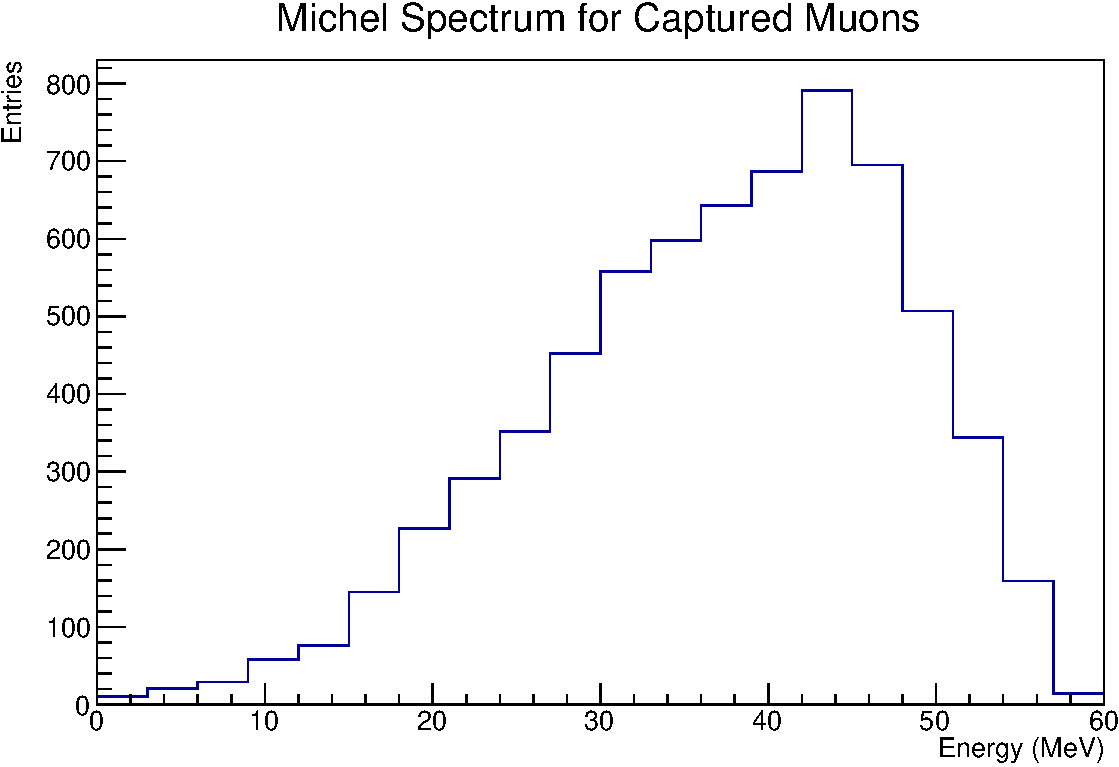
\includegraphics[width=\textwidth]{figures/michel_spec_cap.pdf}
		\caption {Captured Muons.}
		\label{fig:michel_spec_cap}
	\end{subfigure}

	\caption
	[Michel electron energy spectra for free muons and captured muons in liquid
	argon from \protodune{} simulation.]
	{Michel electron energy spectra for free muons and captured muons in liquid
	argon from \protodune{} simulation.}
	\label{fig:michel_spec}

\end{figure}

As discussed in Chapter \ref{ch:energyloss}, the energy loss for electrons in
liquid argon passes from an ionisation dominated regime to a radiation dominated
regime in the tens of MeV region. The crossover point for this transition occurs
at around 30 MeV, close to the peak of the Michel electron spectrum. This
leads to a distinctive signature for Michel electrons in liquid argon 
detectors: a short ($\sim$ 5 cm) track segment is surrounded by a number of 
small radiated energy deposits. Figure \ref{fig:michel_event} shows an example 
of a Michel electron candidate from \protodune{} data, along with labels of 
the key features.

\begin{figure}
	\centering
	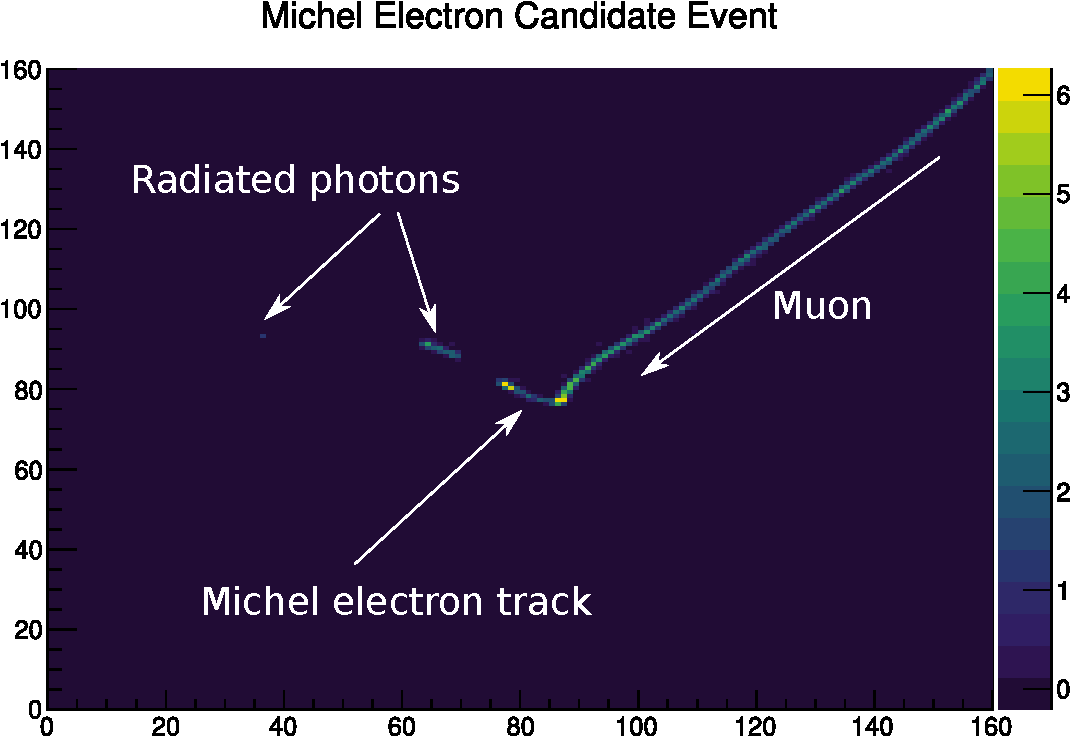
\includegraphics[width=\textwidth]{figures/michel_candidate_labelled.pdf}
	\caption
	[Michel electron candidate event from ProtoDUNE--SP data.]
	{Michel electron candidate event from ProtoDUNE--SP data. The wire vs time
	data in the region of the Michel electron event is shown. The incoming muon,
	initial Michel electron track, and energy depositions from radiated photons
	have been labelled.}
	\label{fig:michel_event}
\end{figure}

One of the main challenges for Michel electron reconstruction in liquid argon is
to successfully associate the radiated energy depositions back to the initial
Michel electron once they have produced ionisation in the detector. Photons have
a radiation length of around 20--30 cm in liquid argon, which is many times
larger than the size of the typical track--like part of the event. Figure
\ref{fig:photon_prop} shows the spectrum of radiated photons from Michel
electron events in \protodune{} simulation, alongside the photon multiplicity
as a function of Michel electron energy. While most of the radiated photons
only carry a small fraction of the Michel electron's energy, in some cases a
single radiated photon can carry a significant fraction of the electron
energy. In addition, around the peak of the Michel electron spectrum ($\sim$
45 MeV) there is a high photon multiplicity and a large spread in the
multiplicity distribution. The combination of these effects leads to a
significant spread in the fraction of radiated energy for Michel electron
events.

\begin{figure}

	\centering

	\begin{subfigure}[b]{\textwidth}
		\centering
		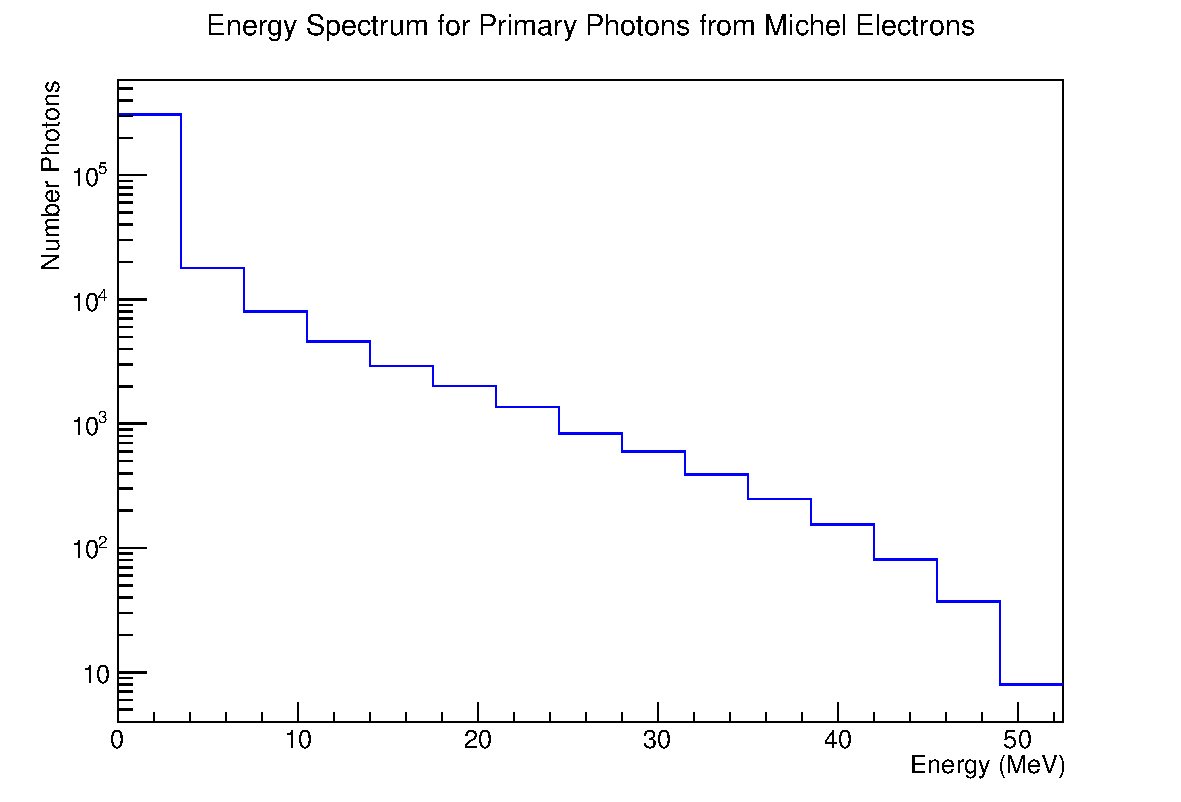
\includegraphics[width=0.9\textwidth]{figures/photon_spec.pdf}
		\caption{Energy spectrum of radiated photons from Michel electron events.}
		\label{fig:photon_spec}
	\end{subfigure}

	\vspace{5mm}

	\begin{subfigure}[b]{\textwidth}
		\centering
		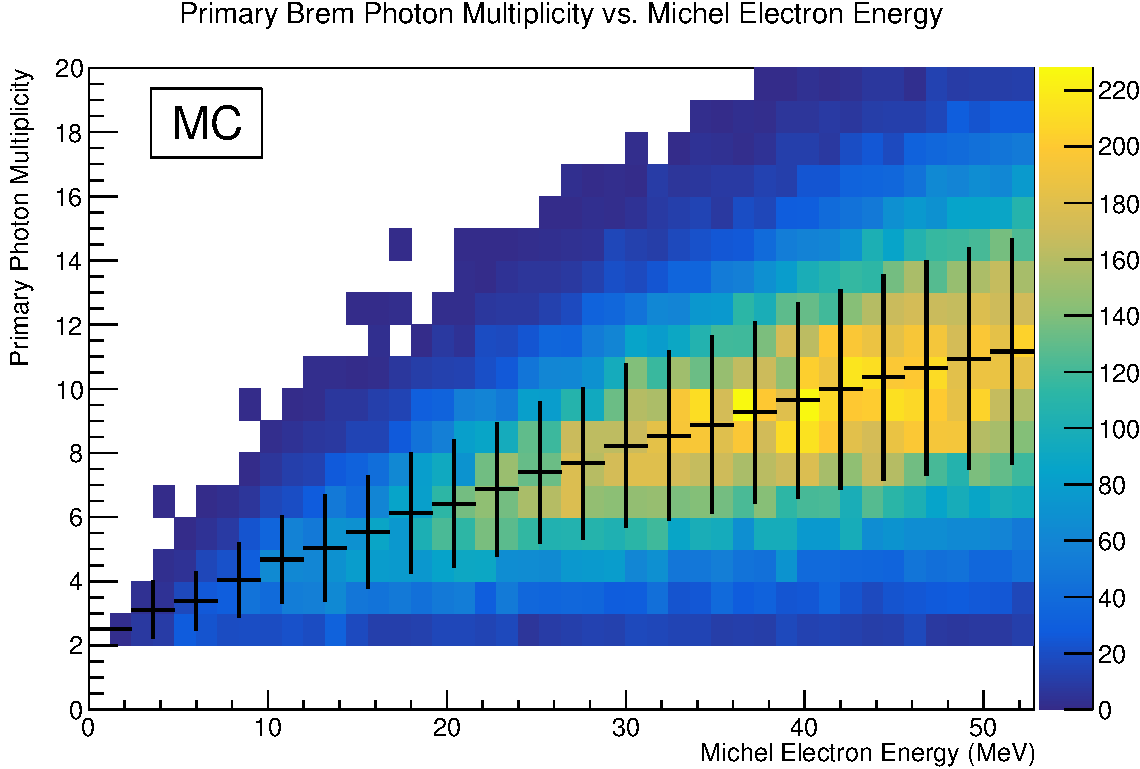
\includegraphics[width=0.9\textwidth]{figures/photon_mult.pdf}
		\caption{Photon multiplicity as a function of true Michel electron energy.
		The distribution is overlaid with a profile of the mean of the distribution,
		the error bars on the profile represent the RMS of a gaussian fit to the
		distribution in each bin.}
		\label{fig:photon_mult}
	\end{subfigure}

	\caption
	[Properties of radiated energy deposits from Michel electrons.]
	{Properties of radiated energy deposits from Michel electrons in \protodune{}
	simulation.}

	\label{fig:photon_prop}

\end{figure}

The energy that is lost into radiated photons is only visible once the photons
interact in the argon to produce secondary electrons, which then ionise the
argon. These secondary electrons are produced over large angles and distances
in the detector when compared to the short Michel electron track, the spatial
distribution of secondary electrons is shown in Figure \ref{fig:photon_geom}.
This shows that the radiated energy deposits are spread over a large area, when
compared to the size of the initial Michel electron track, which is typically
around 5--10 cm. Therefore, any reconstruction algorithm hoping to recover the 
radiated energy, will need to use data from a relatively large volume in order 
to maximise energy recovery.
\begin{figure}
	\centering
	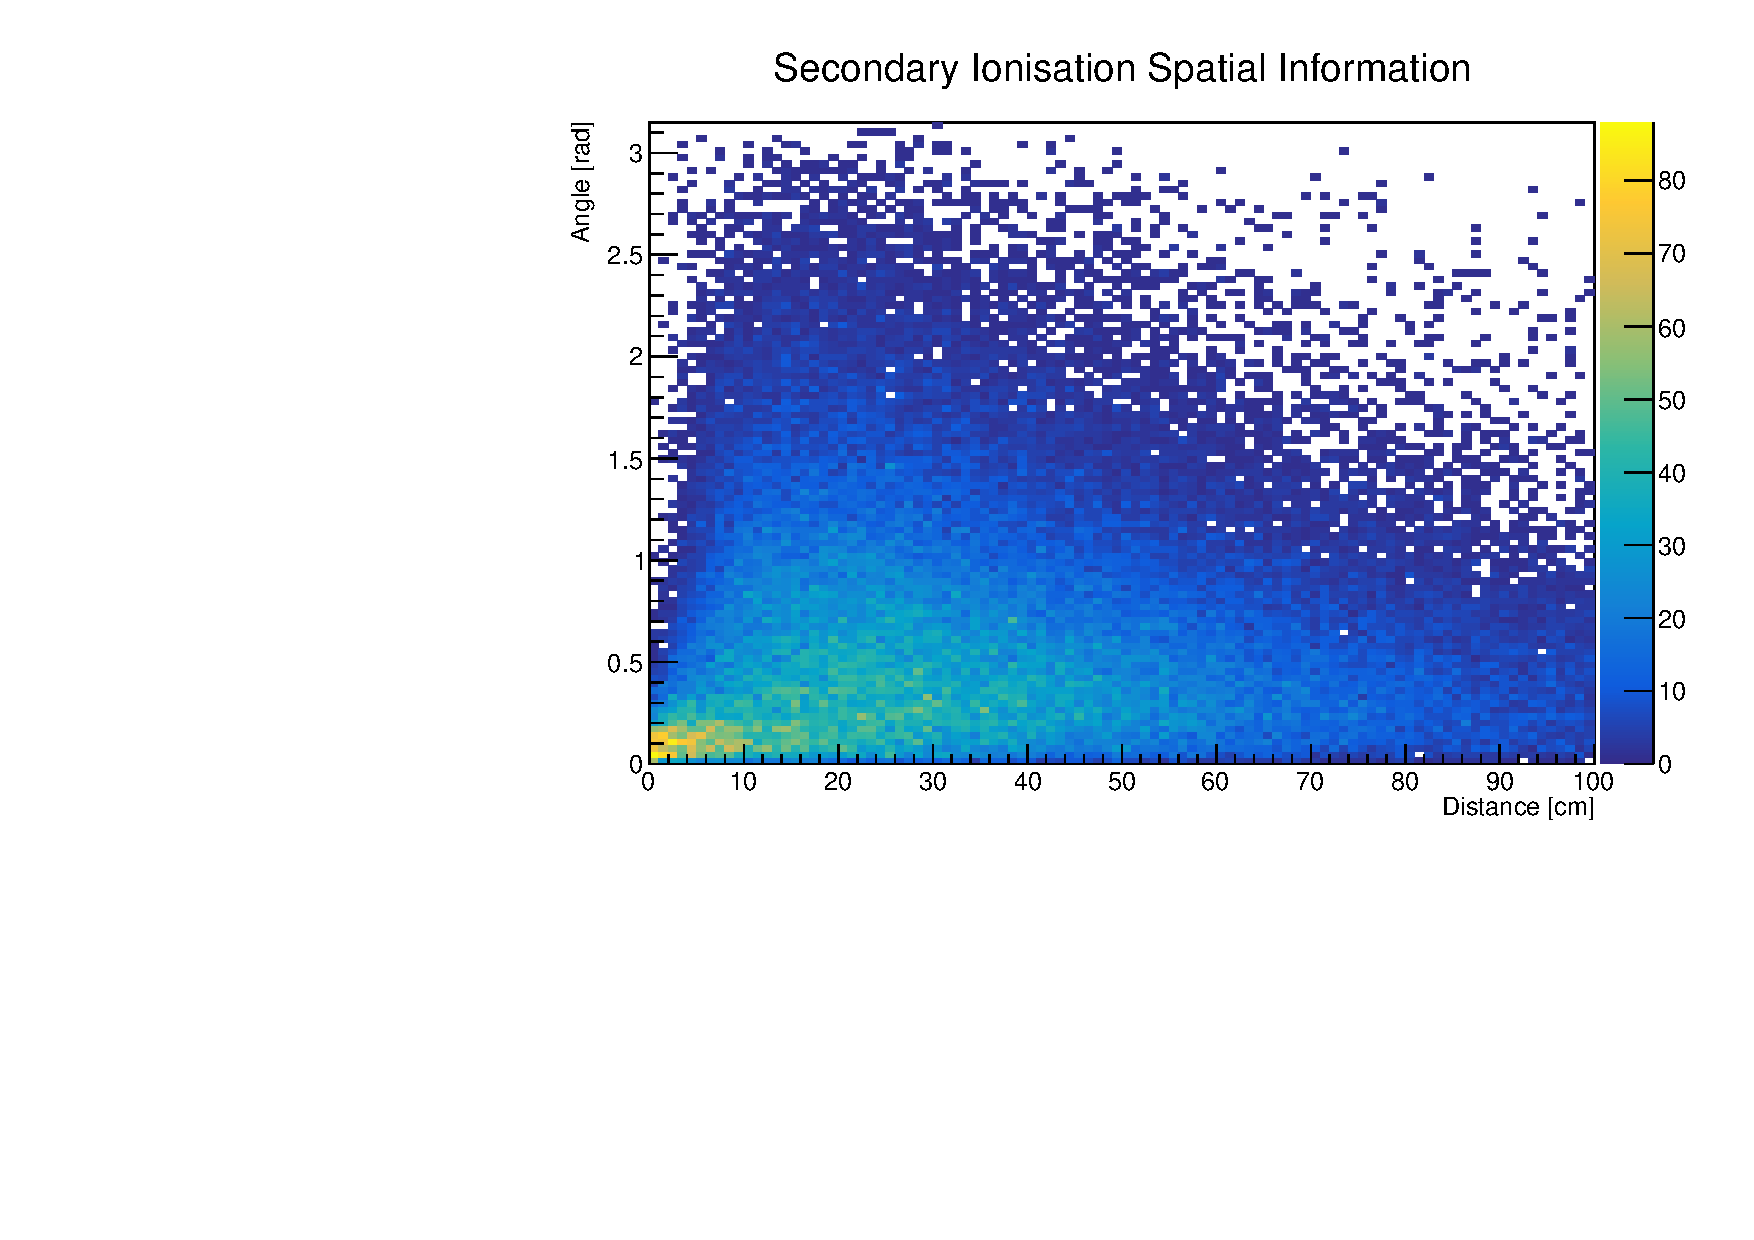
\includegraphics[width=\textwidth]{figures/photon_geom.pdf}
	\caption
	[Spatial distribution of radiated ionisation deposits from Michel electrons.]
	{Spatial distribution of radiated ionisation deposits from Michel electrons.
	This plot shows a 2D histogram of the distance and angle of each radiated
	energy deposition from the primary Michel electron track.}
	\label{fig:photon_geom}
\end{figure}

\noindent
To highlight the impact of the radiated energy deposits, the results of perfect
energy reconstruction were considered in two cases:
\begin{itemize}
	\item Only considering the Michel electron track.
	\item Considering all ionisation energy within some radius and angle of the
		Michel electron track.
\end{itemize}
Figure \ref{fig:michel_track_only} illustrates the considerable increase in
energy collected if radiated energy is considered. The distribution is
significantly narrower, and much more energy is recovered when considering the
energy deposited within a spherical--section of height $40\mbox{ cm}$ and angle
$30^\circ$ of the Michel electron vertex. In addition, the fraction of energy
recovered as a function of Michel electron energy has a more linear
distribution for a collection radius of 40 cm.
\begin{figure}
	\centering

	\begin{subfigure}[b]{\textwidth}
		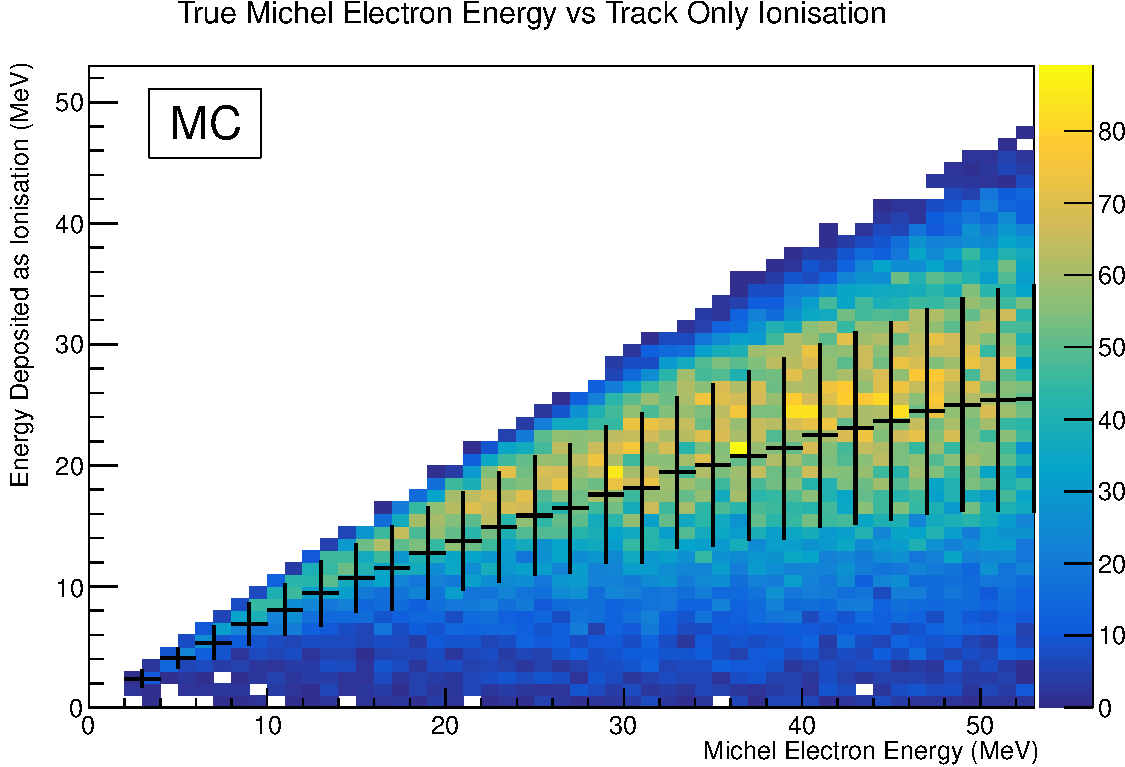
\includegraphics[clip, trim = 0cm 0cm 0cm 1cm, width=\textwidth]{figures/michel_track_only.pdf}
		\caption
		{True collected ionisation energy from the initial Michel electron track
		only.}
		\label{fig:track_only}
	\end{subfigure}

	\vspace{5mm}

	\begin{subfigure}[b]{\textwidth}
		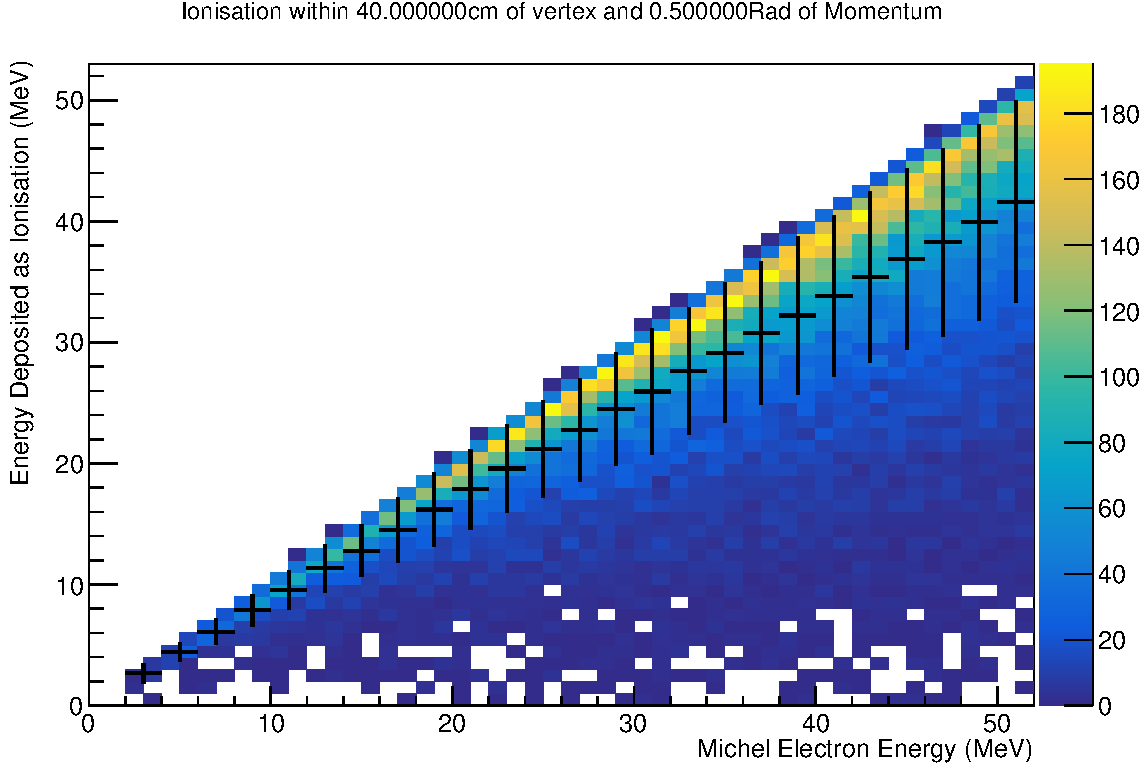
\includegraphics[clip, trim = 0cm 0cm 0cm 1cm, width=\textwidth]{figures/cone_reco.pdf}
		\caption
		{True collected ionisation energy from the initial Michel electron track,
		and any radiated ionisation within a 40 cm spherical--section at a $30^\circ$ 
		opening angle of the initial Michel electron track.}
		\label{fig:cone_reco}
	\end{subfigure}

	\caption
	[Available ionisation energy vs true Michel electron energy for two different
	collection radii.]
	{2D histograms of the true collected ionisation energy vs the true Michel
	electron energy in \protodune{} simulation based on two different collection
	radii.}

	\label{fig:michel_track_only}

\end{figure}

The average fractional energy recovery as a function of collection radius is
shown in Figure \ref{fig:frac_v_radius}, where the error bars represent the RMS
of the distribution. By increasing the collection radius from 0 cm to 40cm,
the average energy recovered is increased from 57\% to 87\%. The RMS of the
fractional energy recovered reduces slightly from 20\% to 16\% across this
range. Therefore, the ratio of the RMS to the mean is reduced from 35\% to 
18\%.
\begin{figure}
	\centering
	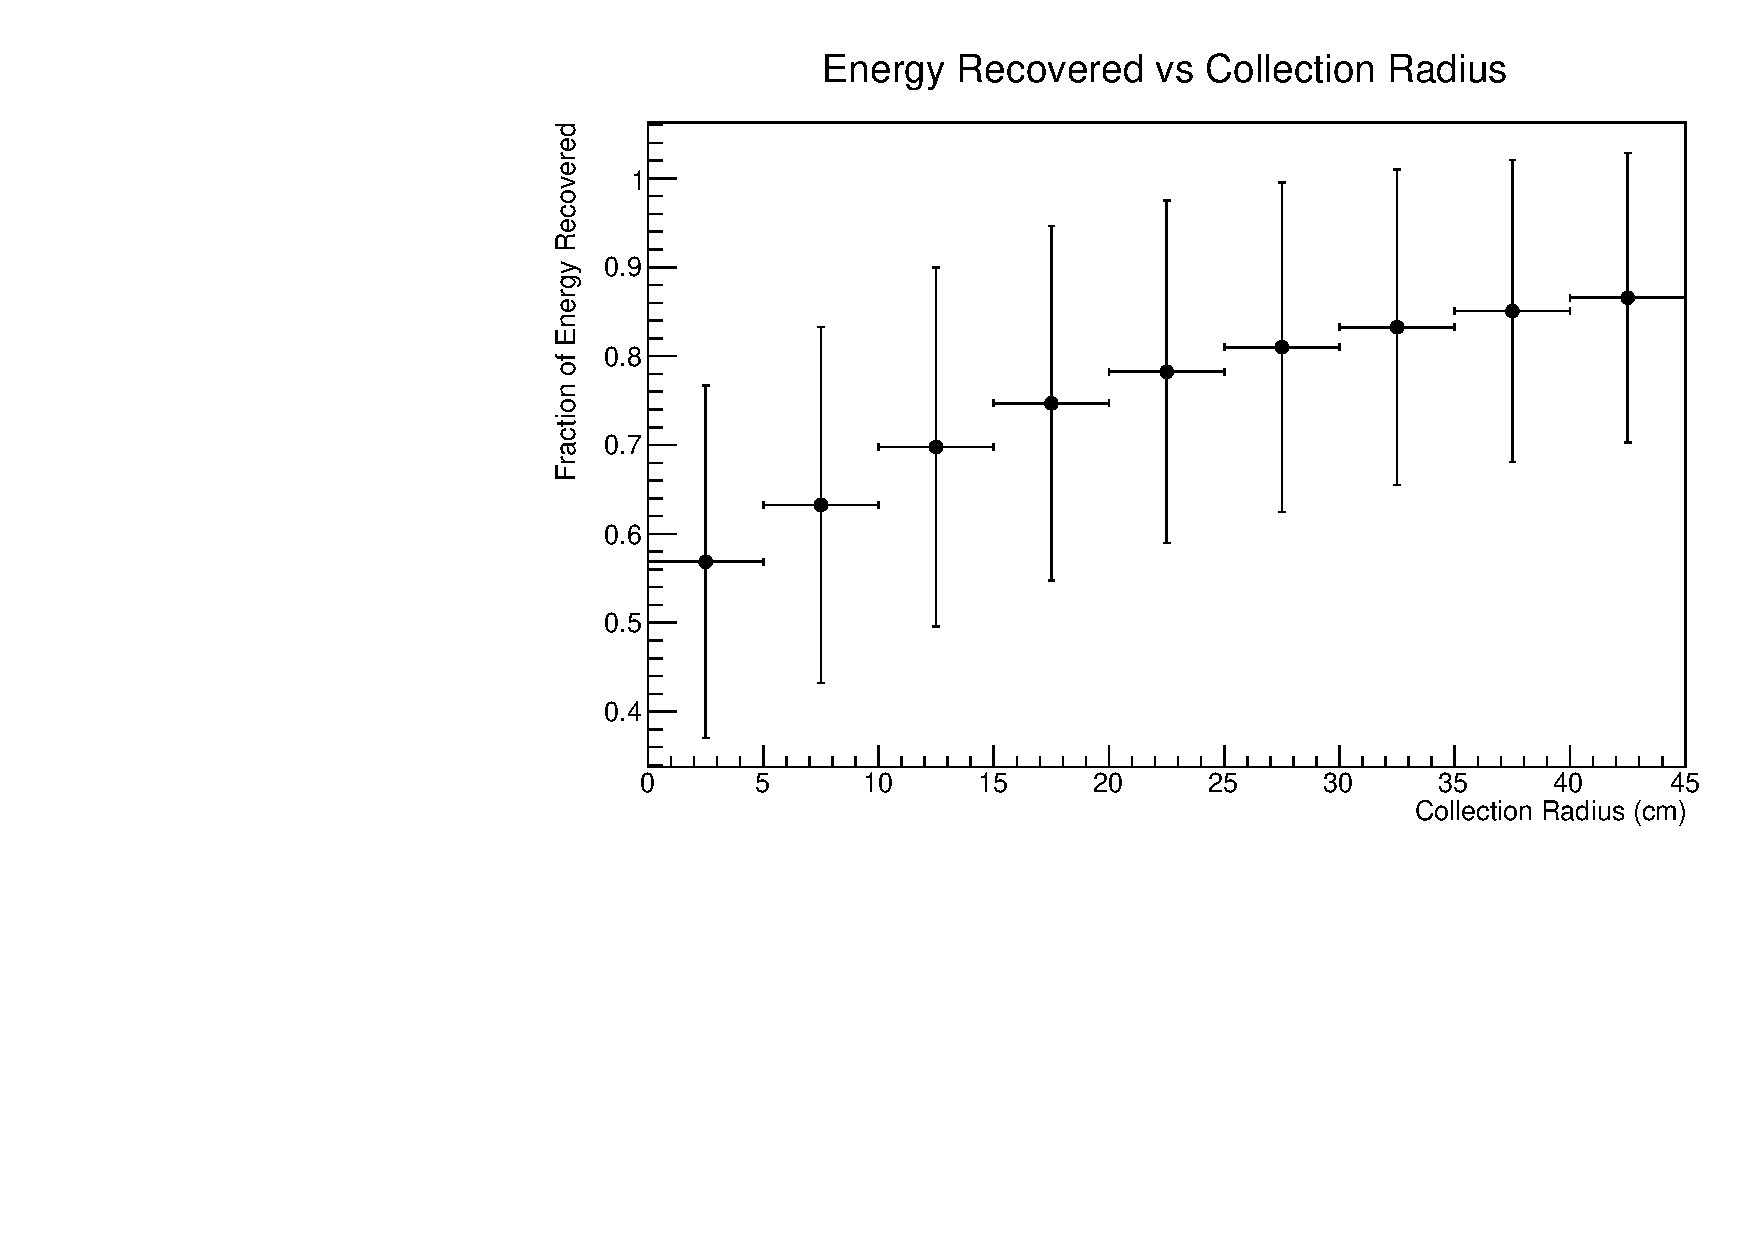
\includegraphics[width=\textwidth]{figures/energy_recovery_v_radius.pdf}
	\caption
	[Fraction of Michel electron energy collected as ionisation vs collection
	radius.]
	{Fraction of Michel electron energy collected as ionisation vs collection
	radius. The error bars here represent the RMS spread of the distribution. }
	\label{fig:frac_v_radius}
\end{figure}

Increasing the collection radius beyond around 30--40 cm gives minimal
improvement in the fractional energy recovery from ionisation. This can been
seen in Figure \ref{fig:40_v_80}, which shows the total true ionisation energy
collected for the case of a 40 cm collection radius and an 80 cm collection
radius. While increasing the collection radius does not significantly increase
the collected ionisation, it was found to impact the purity and efficiency of
reconstruction algorithms. Therefore, the energy reconstruction algorithm
discussed in this chapter considers a 40 cm collection radius when collecting
radiated energy deposits.
\begin{figure}
	\centering
	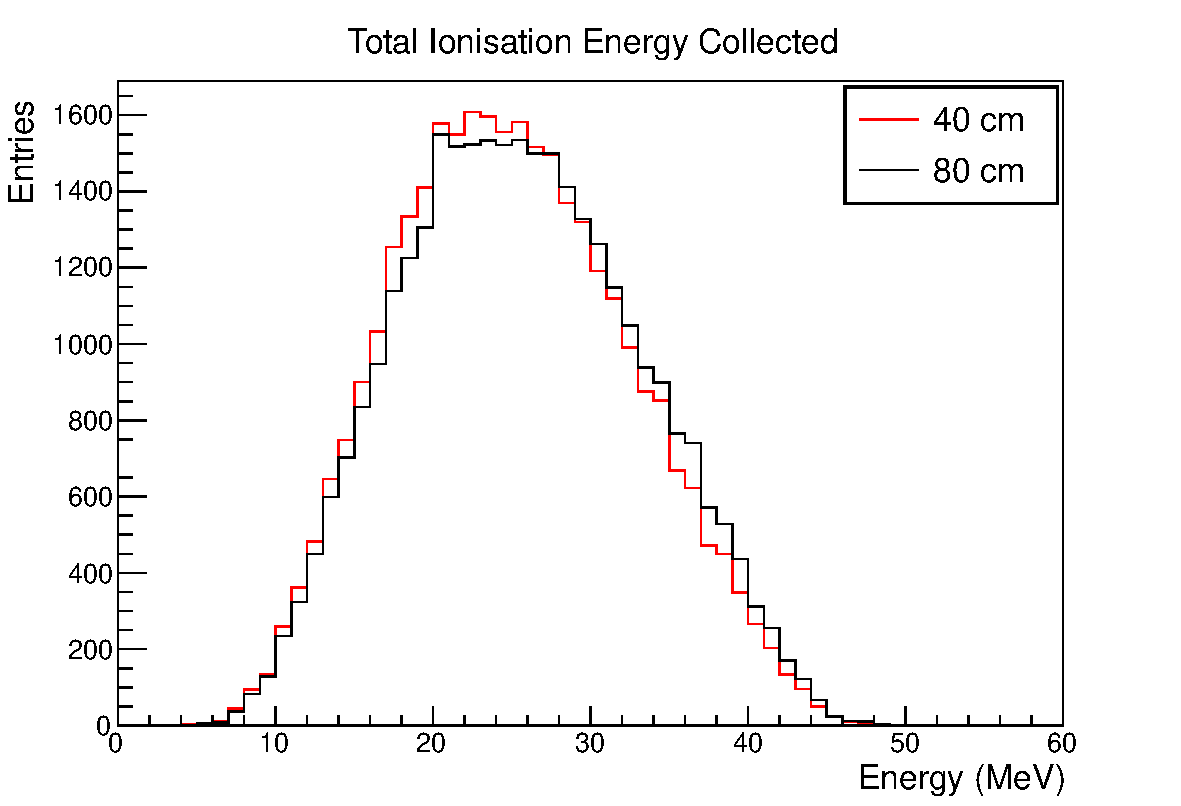
\includegraphics[width=\textwidth]{figures/40_v_80.pdf}
	\caption
	[Total true ionisation energy recovered for a 40 cm collection radius, and an
	80 cm collection radius.]
	{Total true ionisation energy recovered for a 40 cm collection radius, and an
	80 cm collection radius, in red and black respectively.}
	\label{fig:40_v_80}
\end{figure}

The study of \protodune{} simulation presented in this section highlights the 
importance of radiated energy deposits in Michel electron and other 
low--energy electron events. Based on these results, it is clear that to 
reduce energy uncertainties for these events it is important to increase the 
amount of energy collected from radiated photons. The rest of this chapter 
will discuss an algorithm which was developed to tackle this problem, and its 
application on Michel electron events in \protodune{} data.

\section{Michel Electron Event Selection} \label{ME_ES}
In order to select Michel electrons in \protodune{} data, an event selection
algorithm was developed based on combining the results from the hit tagging CNN
from Chapter \ref{ch:chargeid} with clustering performed by the main
\protodune{} reconstruction framework, Pandora. This algorithm has four steps,
which are detailed below.

\subsubsection*{1. Select Primary Tracks}
This step defines the initial sample of muon candidates, which consists of all
primary tracks from the Pandora reconstruction chain.

\subsubsection*{2. Define Michel Electron Candidates}
Based on the sample of muon candidates, a set of Michel electron candidates is
defined. This sample includes any daughter of the muon candidate which satisfies
the following conditions:
\begin{itemize}
	\item It has a start point within 5 cm of the primary track endpoint.
	\item It contains a minimum of 5 reconstructed hits on the collection plane.
\end{itemize}

\subsubsection*{3. Define Best Michel Electron Candidate}
The sample of Michel electron candidates is analysed to select the best Michel
electron candidate. This is the Michel electron candidate with the largest
fraction of Michel--like hits, based on the output of the Michel electron score
from the hit tagging CNN, with a threshold of 0.9. In the case of a tie, the 
candidate with the most hits is chosen.

\subsubsection*{4. Event Selection Cuts}
Events are selected based on the fraction of Michel--like hits in the best 
Michel electron candidate. Figure \ref{fig:michel_like_frac} shows a comparison 
of the fraction of Michel--like hits in Michel electron candidates for 
\protodune{} data and simulation, normalised by the number of muon candidates. 
There is a less good modelling in the fraction of Michel--like hits in 
data for low scores, but a good agreement at higher scores, above around 0.6. 
Events are selected if the Michel electron candidate contains more than 80\% 
Michel--like hits, this threshold was selected by setting a requirement of 
greater than 97.5\% purity on the event selection algorithm in simulation. This 
results in 7.3\% of the best candidates being selected in simulation, and 6.8\% 
in data.

\begin{figure}
	\centering
	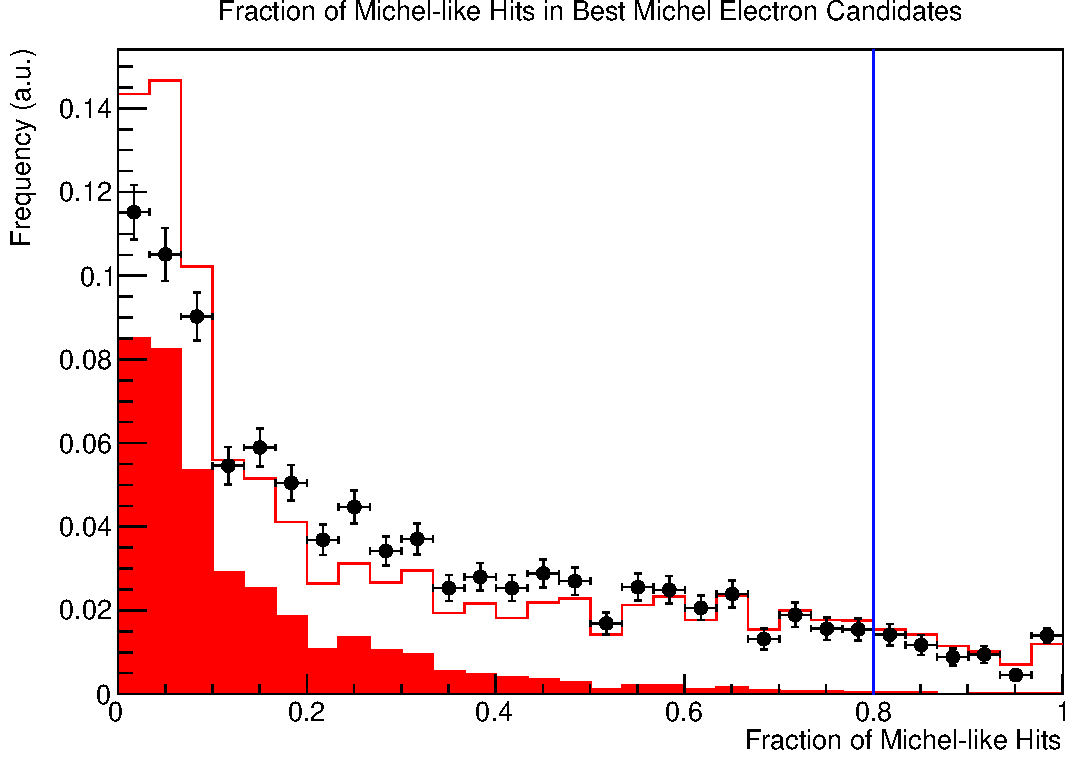
\includegraphics[width=\textwidth]{figures/frac_michel.pdf}
	\caption
	[Fraction of Michel--like hits in the best Michel electron candidate.]
	{Fraction of Michel--like hits in the best Michel electron candidate in data
	and simulation. The red line is the full distribution in simulation, and the
	solid red region represents the background in simulation. The black
	points are the results in data, with statistical error bars only. The vertical
	blue line represents the cut used to select Michel electron candidates as
	Michel electron events, with any candidates containing more than 80\% of
	Michel--like  hits being selected.}
	\label{fig:michel_like_frac}
\end{figure}

\bigskip\noindent
Based on this algorithm, Michel electron events are selected with a
purity of 98\% and an overall efficiency of 6\% in \protodune{} simulation.
Figure \ref{fig:ev_sel_eff} shows the event selection efficiency as a
function on Michel electron energy. The efficiency is reasonably consistent
across the energy range, however, there is a significant reduction for energies
below 5 MeV, which is likely a result of the cut on the minimum number of
collection plane hits. The efficiency is highest for Michel electrons in the
range of 10--40 MeV, and reduces slightly at high energies. At 40--50 MeV,
around the peak of the Michel electron energy spectrum, the efficiency is 
around 5\%.  
\begin{figure}
	\centering
	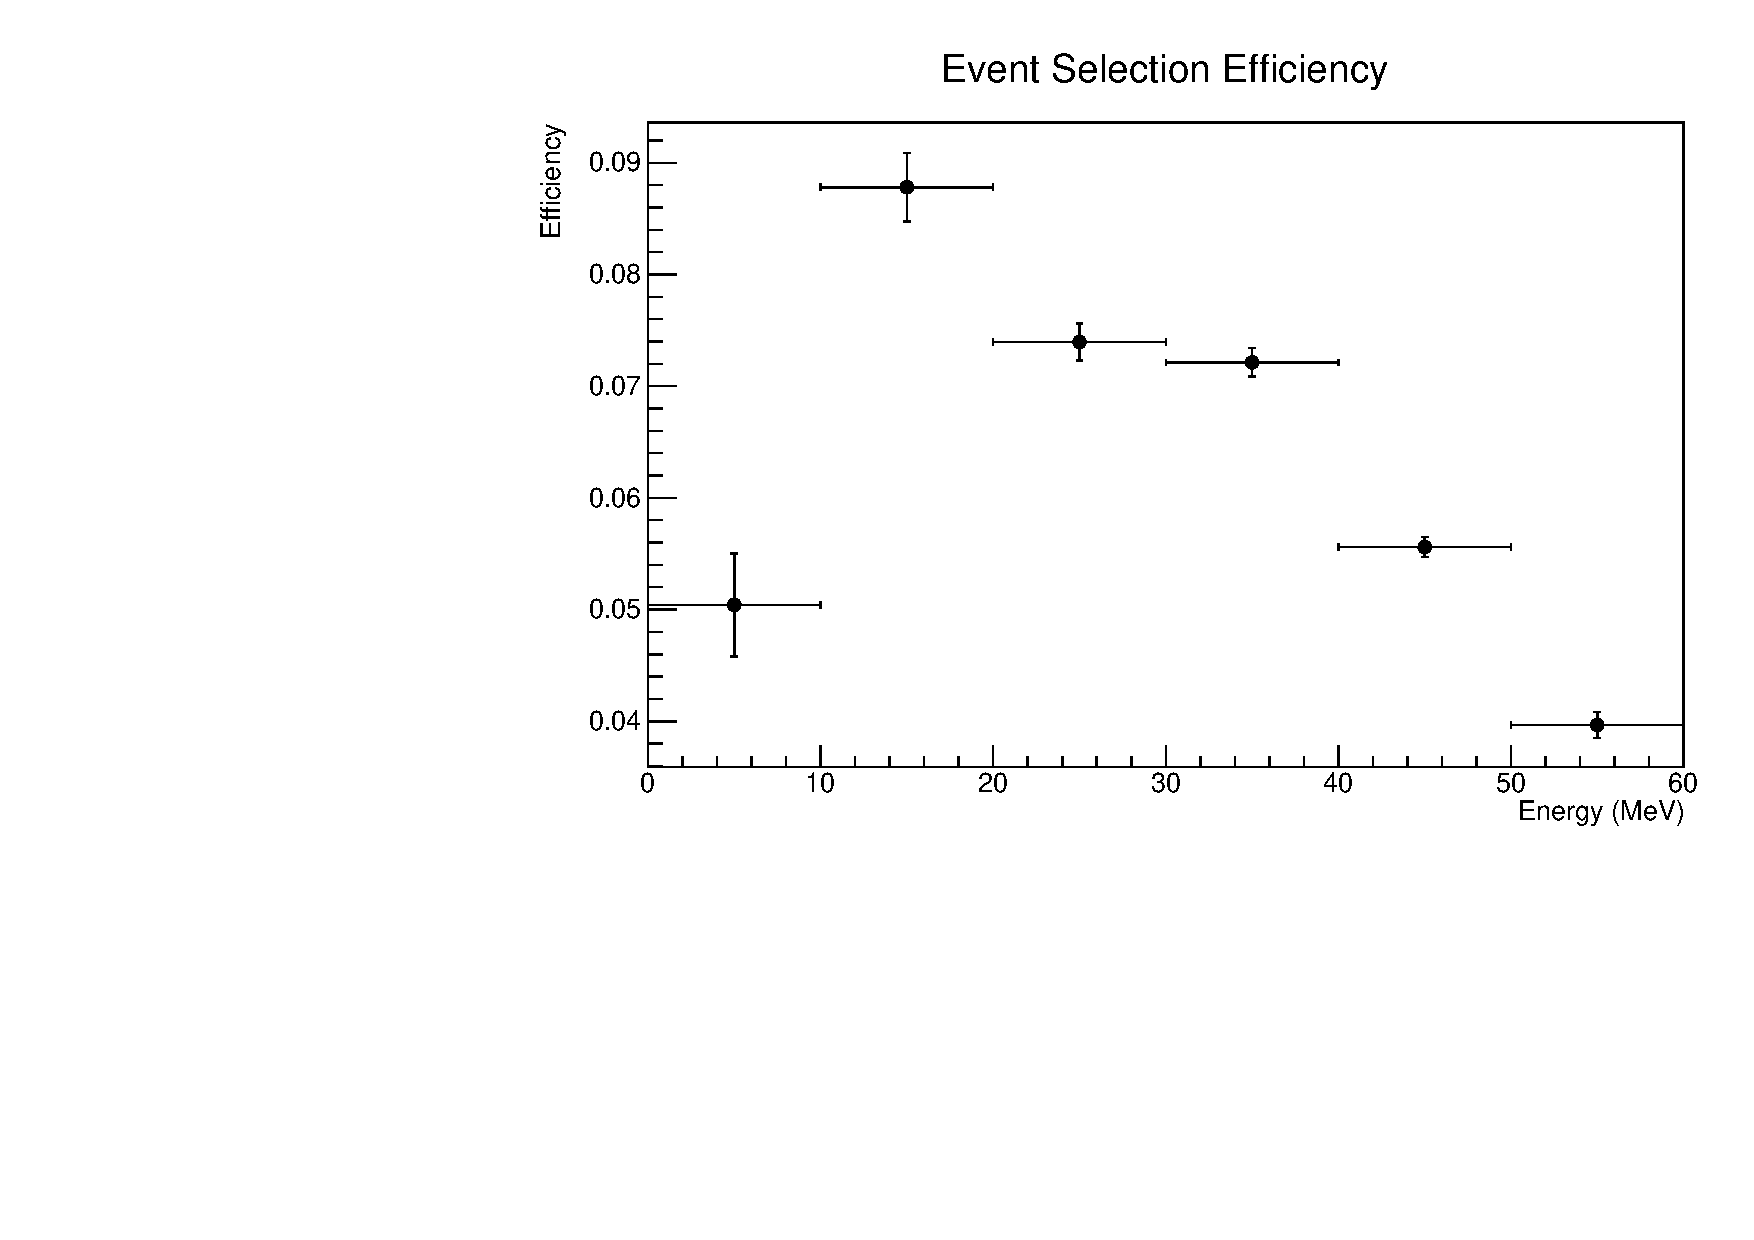
\includegraphics[width=\textwidth, height=0.68\textwidth]{figures/eff_v_energy.pdf}
	\caption
	[Efficiency of Michel electron event selection as a function of energy.]
	{Efficiency of Michel electron event selection as a function of true Michel
	electron energy in \protodune{} simulation, with statistical error bars.}
	\label{fig:ev_sel_eff}
\end{figure}

To accurately estimate the energy of hits during energy reconstruction, the
true time of the Michel electron needs to be known. If not, then the drift 
time of the charge is unknown, and the charge attenuation cannot be estimated.
Therefore, only tracks with reconstructed true time were considered for the 
Michel electron analysis. The spatial and angular distributions of the primary 
muons, normalised by the number of selected muons, are shown in Figure 
\ref{fig:muon_distributions}. There is a reasonable agreement between data and 
simulation for both the spatial and angular distributions.
\begin{figure}

	\centering

	\begin{subfigure}[b]{\textwidth}
		\centering
		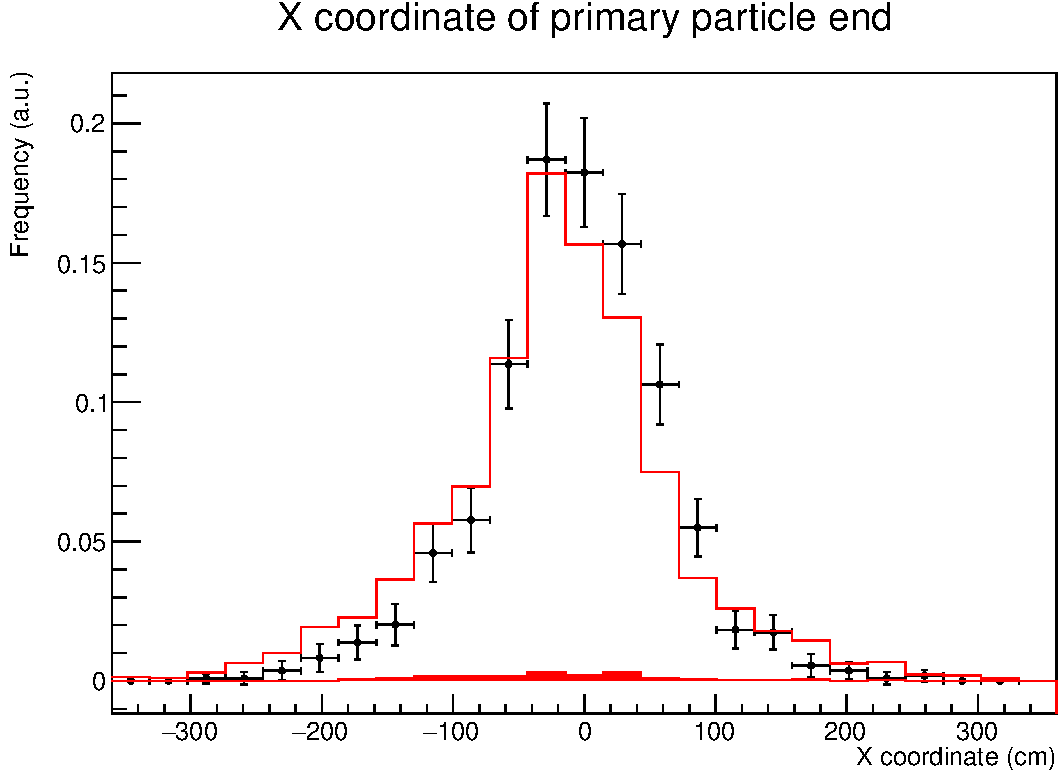
\includegraphics[width=0.484\textwidth]{figures/DataVMC_primary_EndX.pdf}
		\hfill
		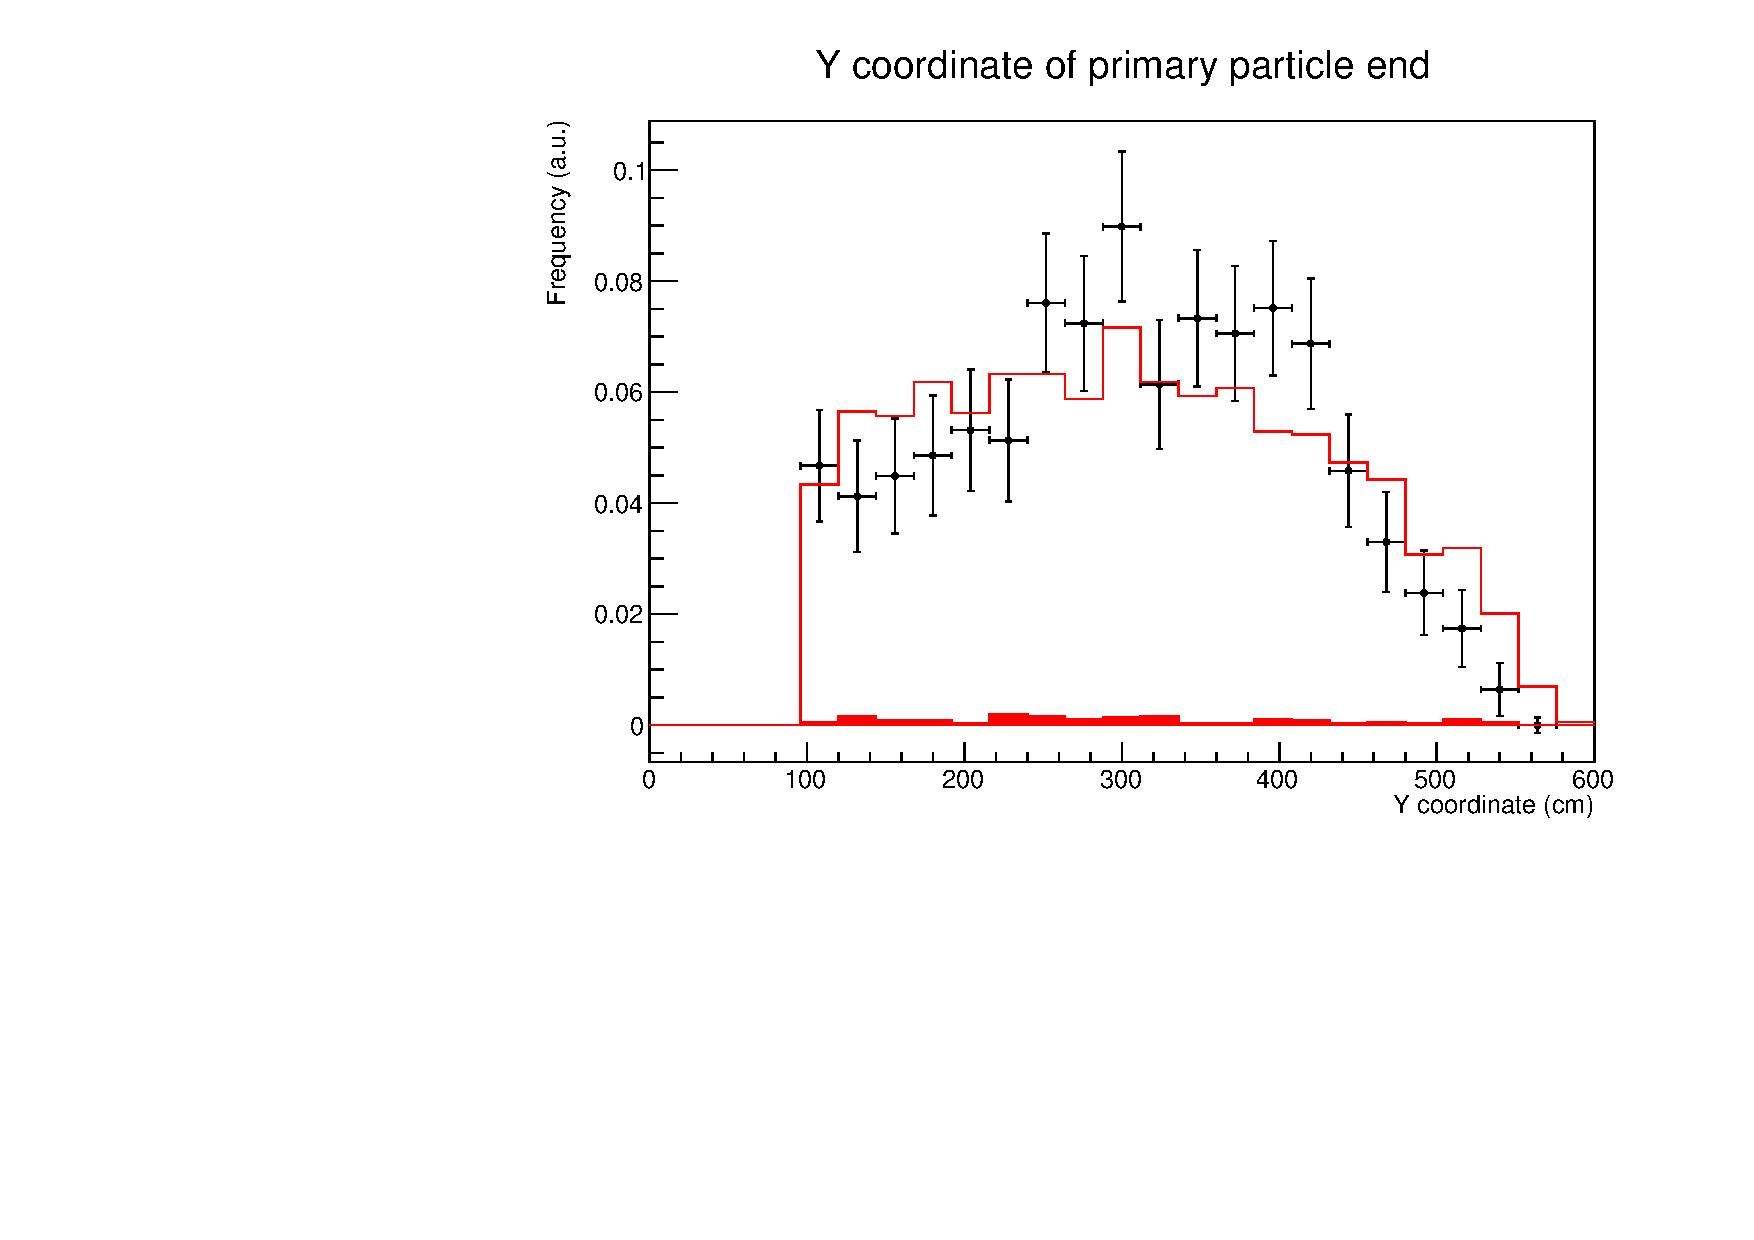
\includegraphics[width=0.484\textwidth]{figures/DataVMC_primary_EndY.pdf}
		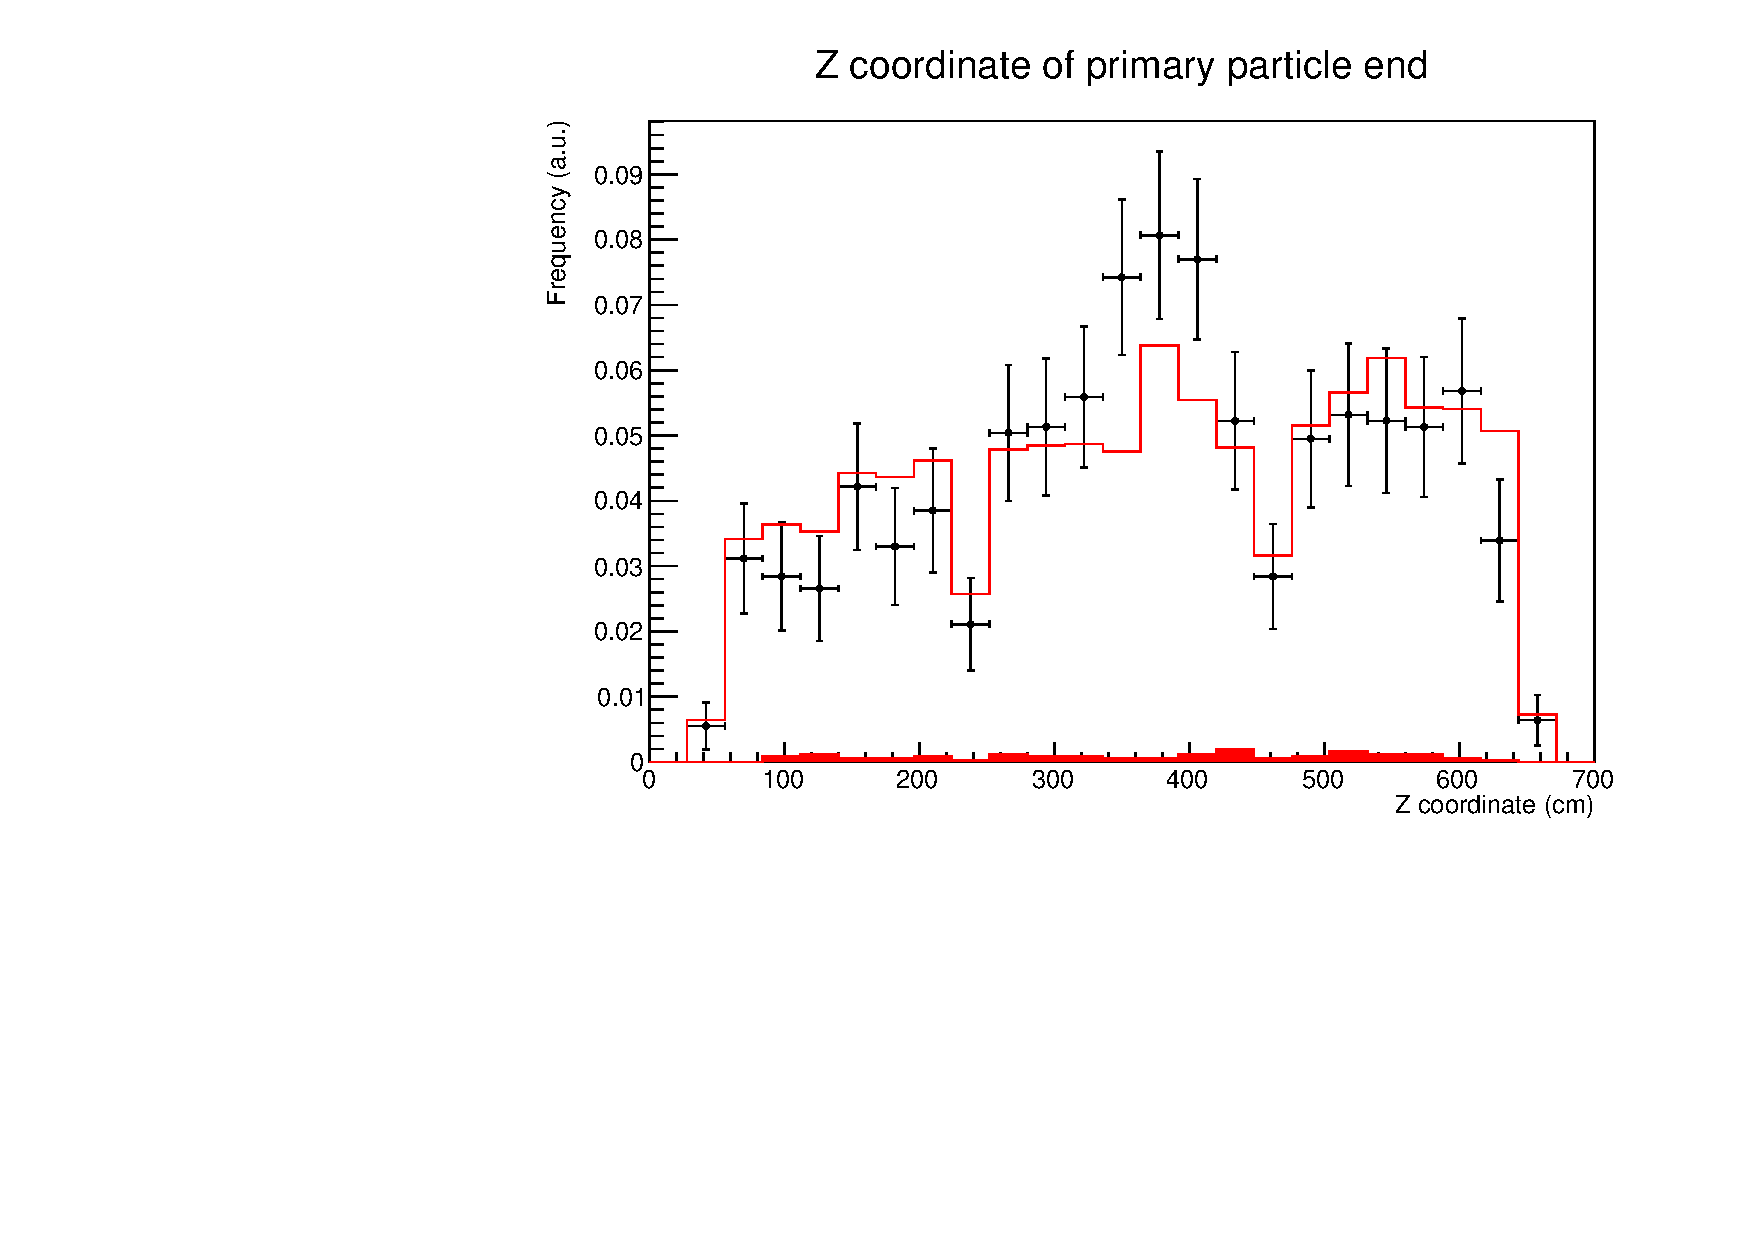
\includegraphics[width=0.484\textwidth]{figures/DataVMC_primary_EndZ.pdf}
		\caption {Primary muon end--points: X (drift), Y (vertical), Z (beam).}
		\label{fig:muon_endpoints}
	\end{subfigure}

	\begin{subfigure}[b]{\textwidth}
		\centering
		\vspace{5mm}
		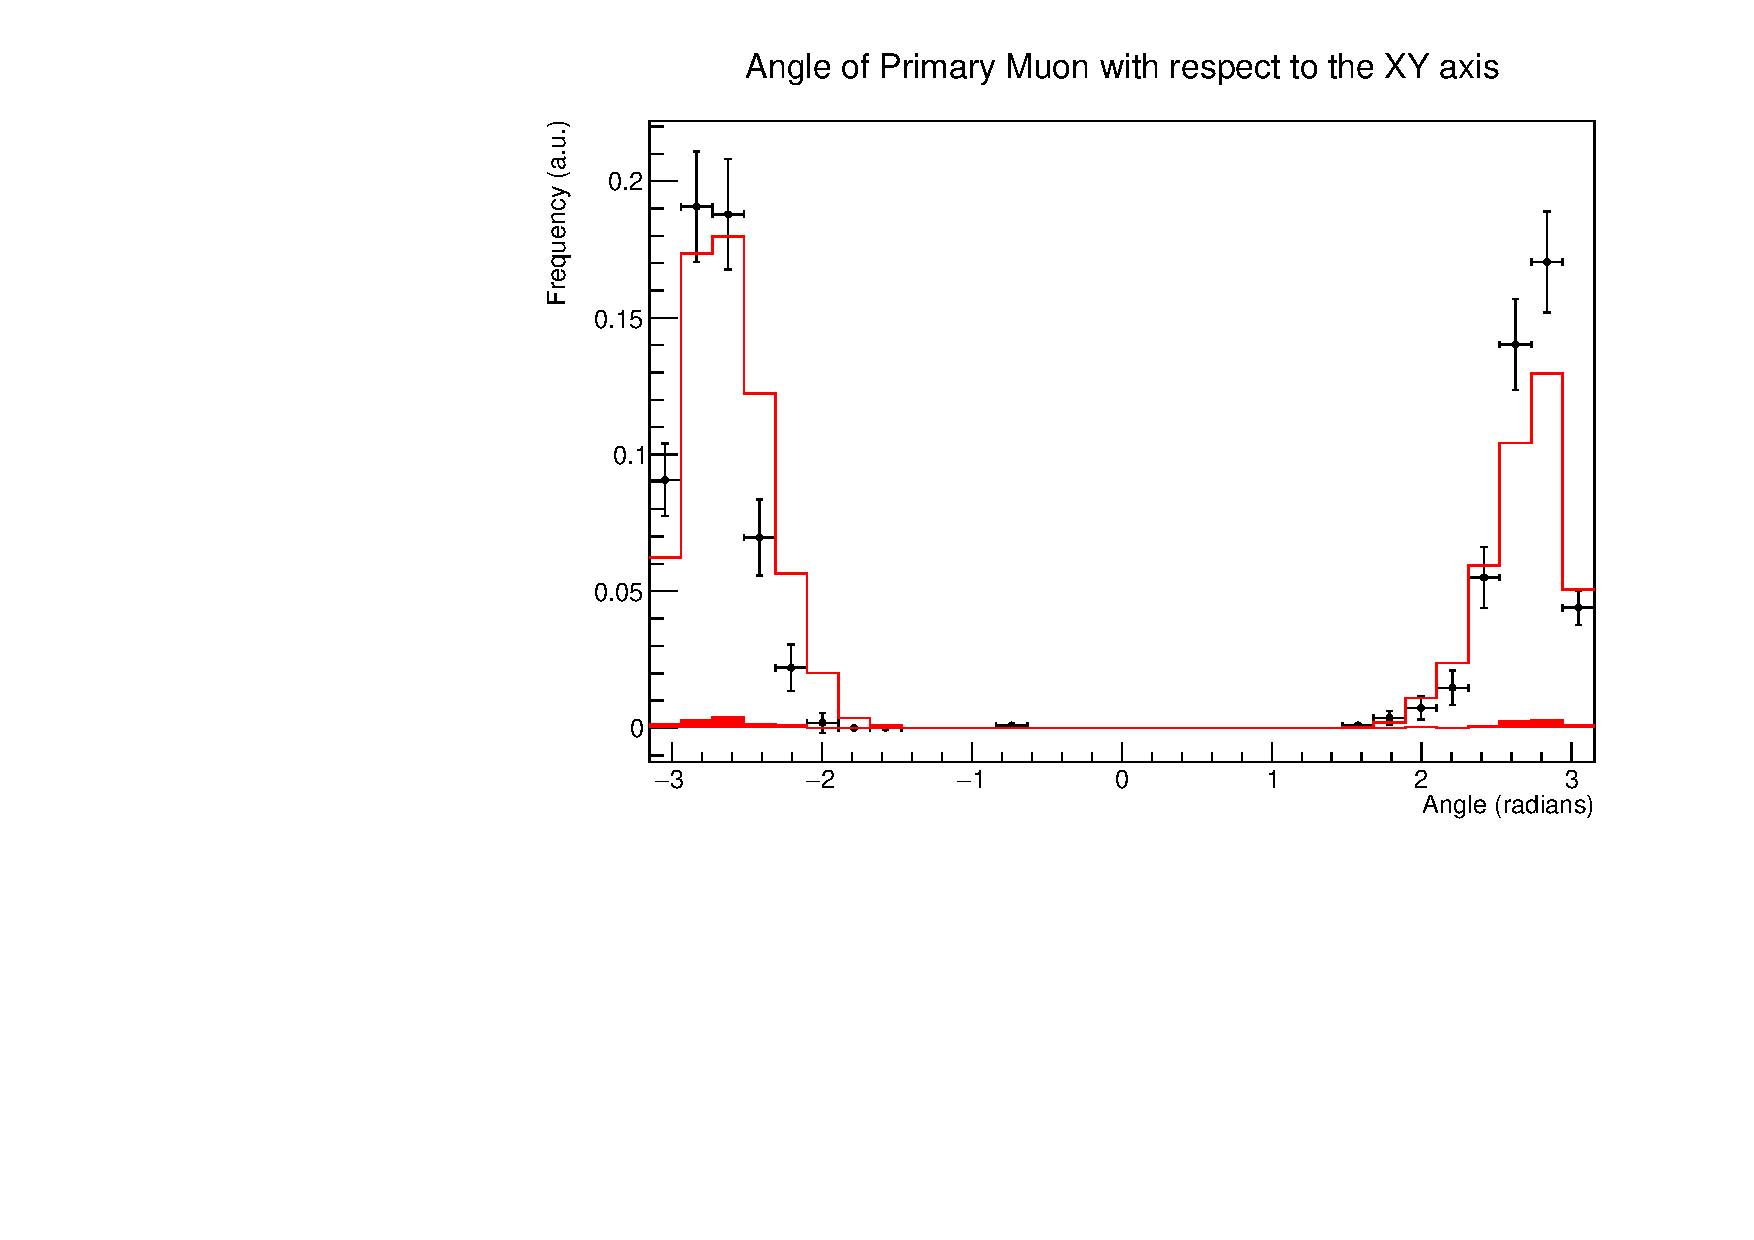
\includegraphics[width=0.484\textwidth]{figures/DataVMC_angle_xy.pdf}
		\hfill
		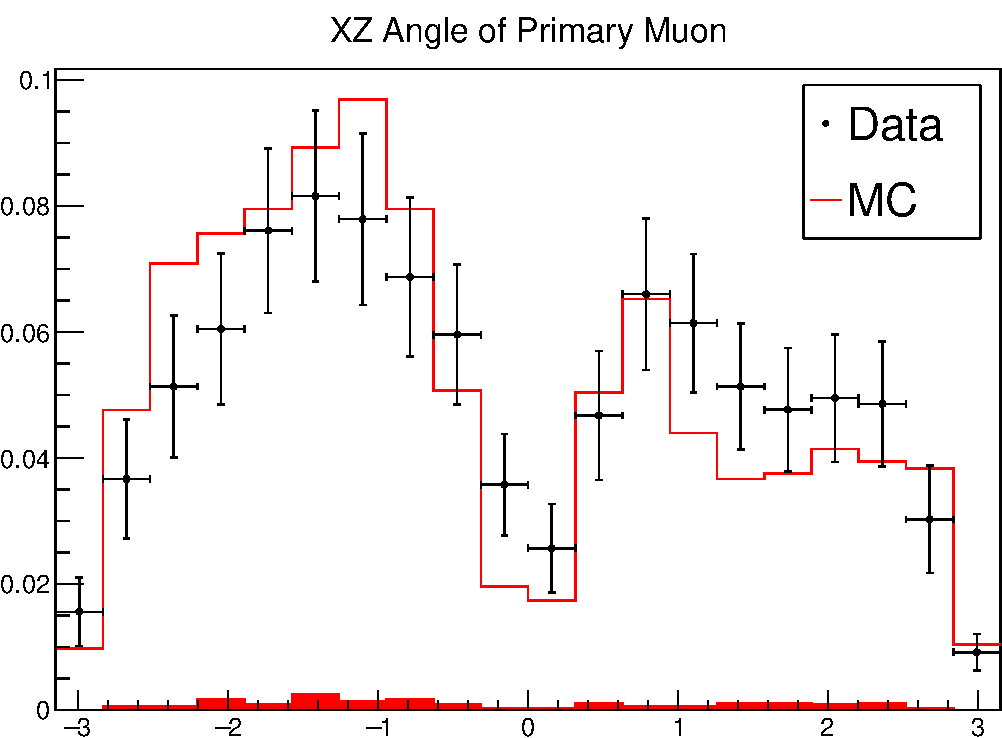
\includegraphics[width=0.484\textwidth]{figures/DataVMC_angle_xz.pdf}
		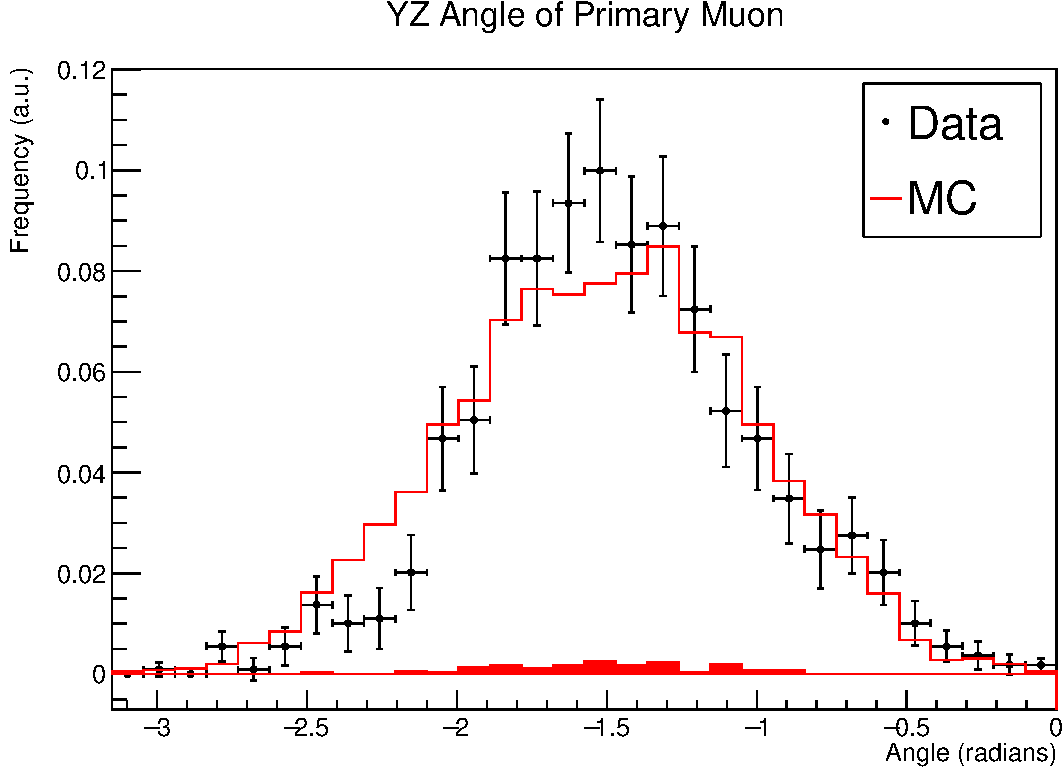
\includegraphics[width=0.484\textwidth]{figures/DataVMC_angle_yz.pdf}
		\caption {Primary muon angular distributions.}
		\label{fig:muon_angles}
	\end{subfigure}


	\caption
	[Spatial and angular distributions for primary muons associated with selected
	Michel electrons.]
	{Spatial and angular distributions for primary muons associated with selected
	Michel electrons, with statistical error bars.}

	\label{fig:muon_distributions}

\end{figure}

\section{Michel Electron Energy Reconstruction} \label{ME_R}

To reconstruct the energy of Michel electrons in liquid argon the relevant hits
must first be selected. The reconstructed ionisation energy for the Michel
electron is the sum of the reconstructed ionisation energy for all of the
selected hits. This section will detail a hit selection algorithm based on a 
type of convolutional neural network called a U--ResNet, which returns hit 
selection maps for the Michel electron energy reconstruction. This algorithm 
is used to select Michel electron hits with a high purity and efficiency, and 
the resulting reconstructed energy spectrum is used to estimate the energy 
resolution of \protodune{} for electrons in the tens of MeV range.

\subsection{Michel Electron Hit Tagging with a U--ResNet}

A U--ResNet is a type of convolutional neural network which is designed to 
perform semantic segmentation of images. The U--ResNet network architecture 
was first developed for biomedical image segmentation\cite{ronneberger2015u}. 
In semantic segmentation the aim is to return a map of pixels which correspond 
to the areas of interest; the output of the network is the same dimension as 
the input with a one--to--one correspondence between input pixels and output 
pixels. The architecture used for the hit selection algorithm is shown in 
Figure \ref{fig:unet_arch}. During the first half of the network architecture 
the resolution of the output is decreased, this is analogous to many 
conventional CNNs, and it is during this phase the network learns about the 
content of the image. The second phase of the architecture allows the 
U--ResNet to rebuild the locations of different learned features within the 
initial image. This is achieved by passing the details of previous layers to 
the network, through residual connections, allowing the resolution of the 
output map to be slowly increased back to the original resolution.

The network architecture used for the Michel electron reconstruction is shown in
Figure \ref{fig:unet_arch}. The network consists of a repeating structure, which
contains the following key components:
\begin{itemize}
	\item Convolutional blocks, which contain multiple convolutional layers.
	\item Pooling layers for downscaling in the first half of the network.
	\item Residual connections and up--sampling in the second half of the network.
\end{itemize}
The convolutional blocks each contain three convolutional layers, which is
shown in Figure \ref{fig:conv_block}. These take the form of inception
units\cite{Szegedy2015} with leaky ReLU activation functions; a schematic of
the inception units is shown in Figure \ref{fig:unet_inception}. During the
first half of the network, maximum pooling is used to downsample the size of
the feature maps, which reduce by a factor of two in each max pooling layer.
Then, during the second half of the network, the up--sampling layers increase
the resolution of the feature maps by a factor of two, such that the output of
the network has the same resolution as the input. The residual connections
from early layers, are combined with the up--sampled feature maps, to allow
the network to reconstruct the location of the learned features. As with the
CNN from the previous chapter, both dropout and early--stopping are
implemented to prevent over--fitting.

In the Michel electron case, the aim of the network is to return a map of all
ionisation energy deposits from the Michel electron, including the initial
track and any secondary deposits from radiated photons. The inputs and outputs
are two dimensional images of the location of reconstructed hits, centered on
the selected Michel electron candidate. The amplitude of each input pixel is
given by the integrated charge of any reconstructed hits within the pixel. For
the true output images the pixels have an amplitude of 1 if they contain a
Michel electron hit, and 0 otherwise. Only data from the collection plane is
used, because there is a higher signal to noise ratio on these wires.

The $F_\beta$ metric\cite{VanRijsbergenC.J.1975Ir} was used as the loss
function for the U--ResNet. This loss is a generalised version of the $F_1$
metric discussed in Chapter \ref{ch:chargeid}, which allows for the relative
importance of purity and efficiency to be tuned,
\begin{equation*}
	F_\beta = \left( 1 + \beta^2\right) \frac{\mbox{purity} \cdot
	\mbox{efficiency}}{\left(\beta^2 \cdot \mbox{purity}\right) +
	\mbox{efficiency}}.
\end{equation*}
This loss rewards the network for selecting as many correct hits as possible
(high efficiency), while penalising it for selecting more hits that necessary 
(low purity). The $F_\beta$ score lies between 0 and 1, with a score of 1 
corresponding to a perfect match. The $\beta$ parameter was chosen to be 2, 
such that efficiency was considered to be more important than purity. This was 
found to improve the performance of the Michel electron reconstruction in terms 
of energy resolution and bias, however, no extensive optimisation of $\beta$ was
performed.

\begin{figure}

	\centering

	\begin{tabularx}{\textwidth}{cX}
		\begin{subfigure}[b]{0.40\textwidth}
			\centering
			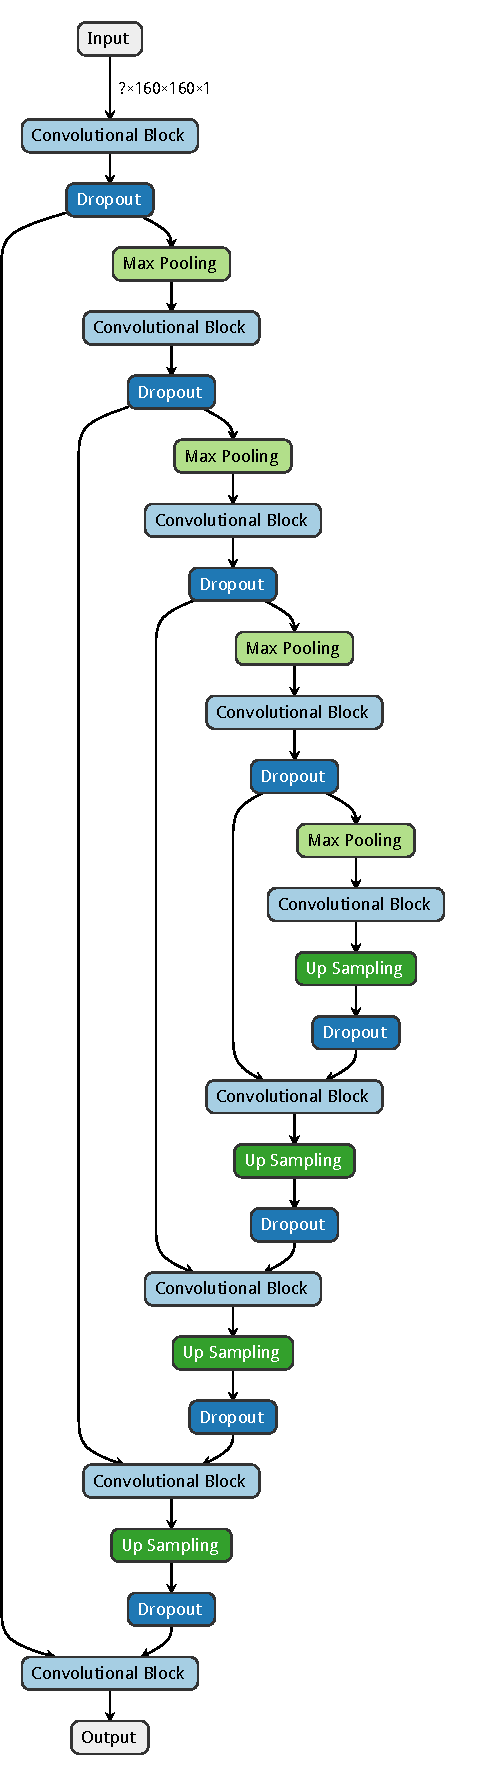
\includegraphics[height=0.91\textheight]{figures/unet_arch.pdf}
			\caption {Overall structure.}
			\label{fig:unet_structure}
		\end{subfigure}
		&
		\begin{tabular}[b]{c}
			\begin{subfigure}[b]{0.5\textwidth}
				\centering
				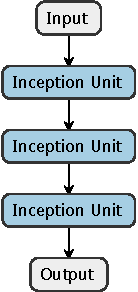
\includegraphics{figures/conv_block.pdf}
				\caption {Convolutional block.}
				\label{fig:conv_block}
			\end{subfigure} \\
			\vspace{10mm} \\
			\begin{subfigure}[b]{0.5\textwidth}
				\centering
				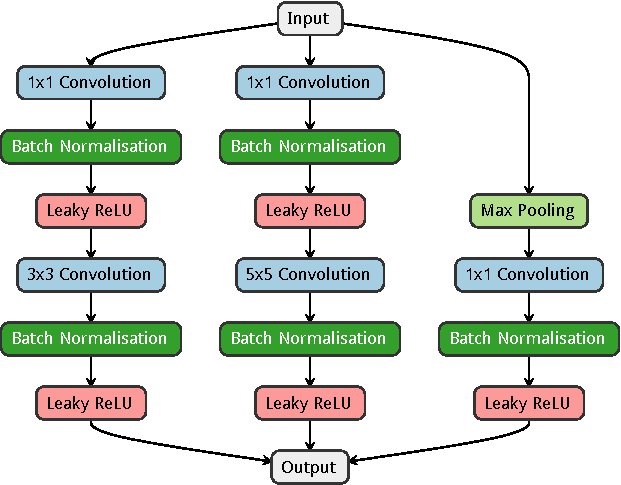
\includegraphics[width=\textwidth]{figures/inception_arch.pdf}
				\caption {Inception unit.}
				\label{fig:unet_inception}
			\end{subfigure}
		\end{tabular}
	\end{tabularx}

	\caption
	[U--ResNet CNN architecture used to select Michel electron ionisation energy
	deposits.]
	{U--ResNet CNN architecture used to select Michel electron ionisation energy
	deposits. Visualisation adapted from the output of the Netron neural network
	viewer\cite{netron}.}

	\label{fig:unet_arch}
\end{figure}

The datasets for the training process were generated from a full simulation of
the \protodune{} detector under beam operation, including both cosmic--ray and
beam particles. The images produced contain the location and integrated charge
for each hit within the image window. The training data was split into training, 
test, and validation sets in the ratio 80:10:10. In total around 15,000 images 
were used in the combined training, test, and validation datasets.

As with the hit tagging CNN discussed in Chapter \ref{ch:chargeid}, the 
training and validation scores were monitored throughout training using 
TensorBoard. The weights of the network were saved after each epoch, and the 
final weights were those from one epoch before the validation score first 
increased. Figure \ref{fig:unet_loss} shows the evolution of the loss over 
time, along with a vertical line representing the loss at which the weights 
were chosen.
\begin{figure}
	\centering
	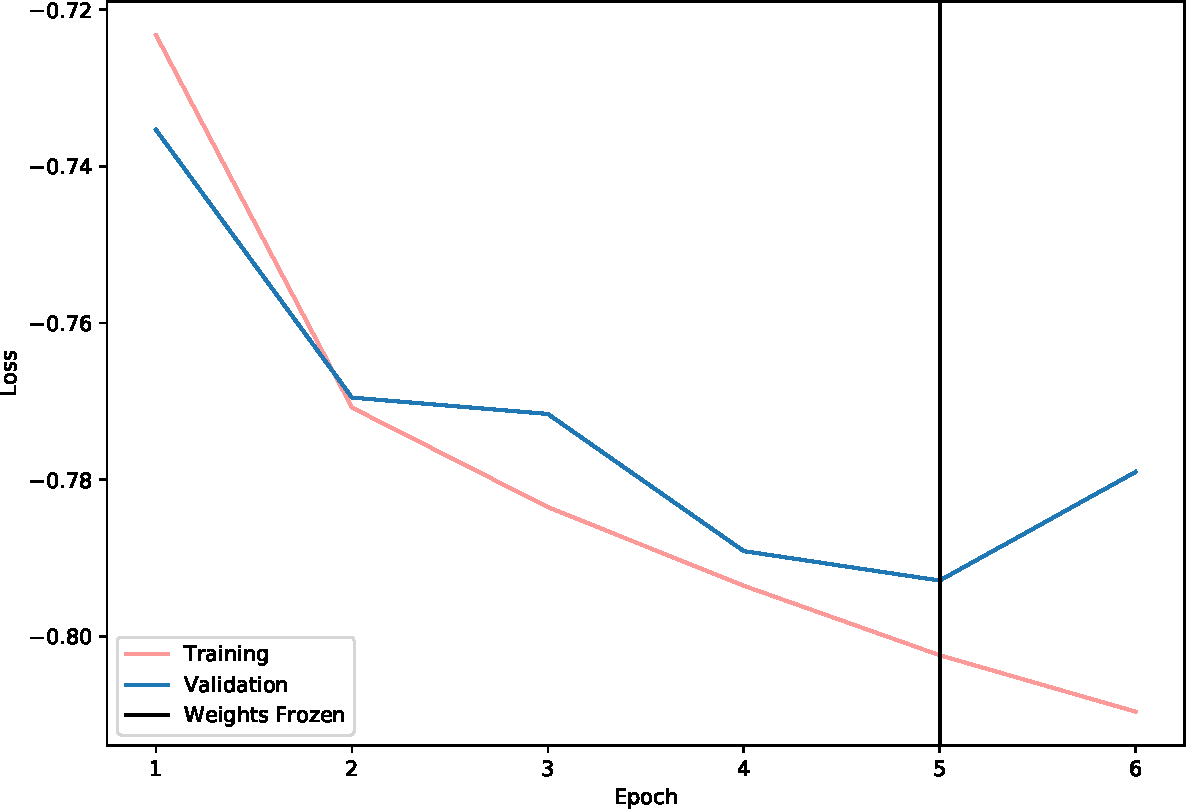
\includegraphics[width=\textwidth]{figures/unet_loss.pdf}
	\caption
	[U--ResNet training and validation loss as a function of epoch.]
	{U--ResNet training and validation loss as a function of epoch. The weights were
	frozen based on an early stopping algorithm, which is demonstrated by the
	vertical black line.}
	\label{fig:unet_loss}
\end{figure}

A demonstration of the output of the U--ResNet is given in Figure
\ref{fig:unet_example} which shows the input, output, and truth images for an
event from \protodune{} simulation.
\begin{figure}
	\centering

	\begin{subfigure}[b]{0.5\textwidth}
		\centering
		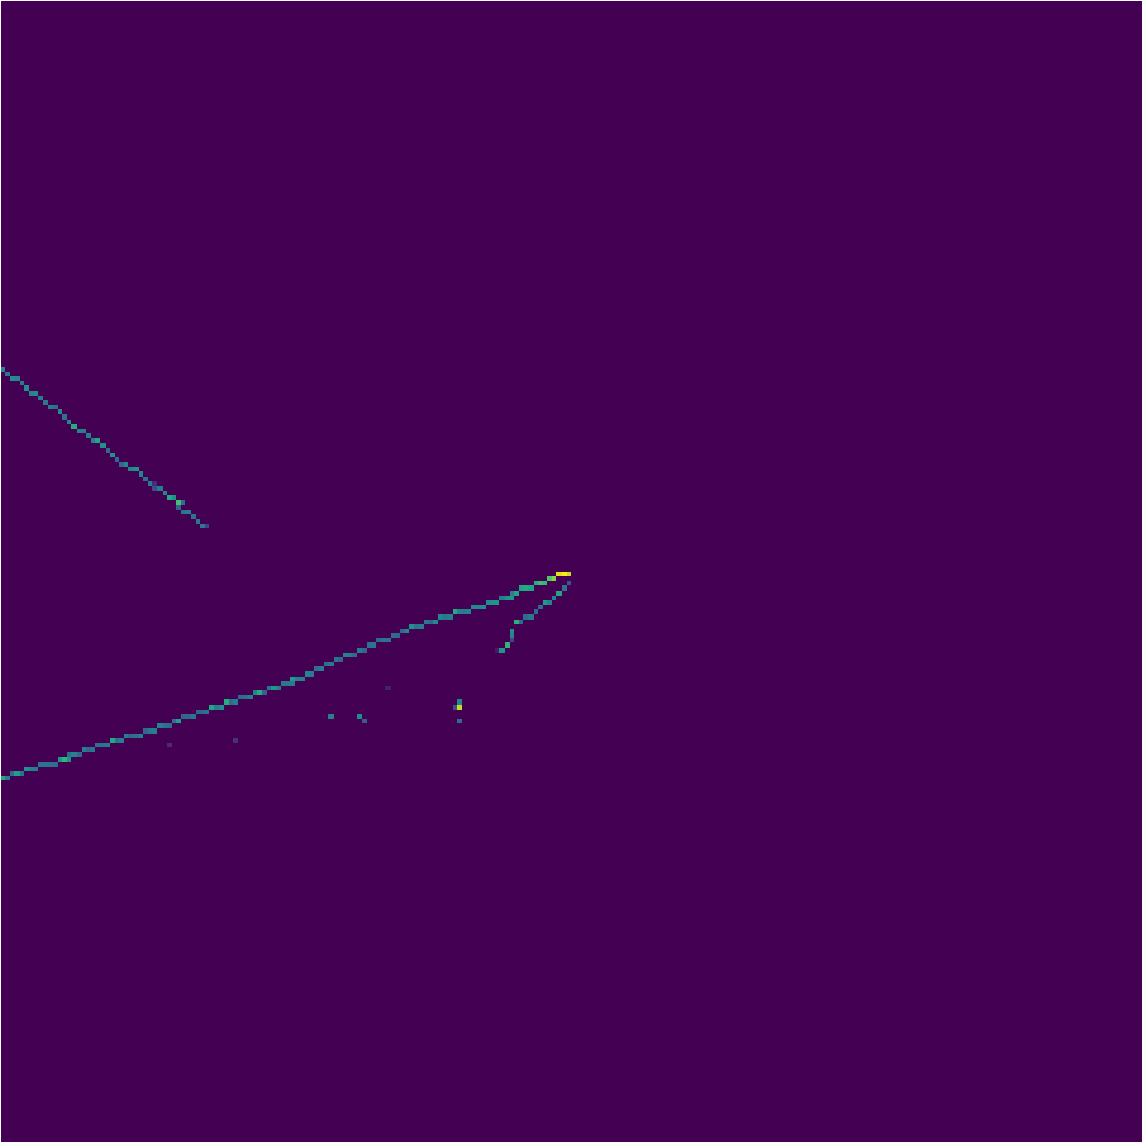
\includegraphics[width=\textwidth]{figures/unet_example_in.pdf}
		\caption {Input.}
		\label{fig:unet_example_in}
	\end{subfigure}

	\begin{tabularx}{\textwidth}{cc}
		\begin{subfigure}[b]{0.49\textwidth}
			\centering
			\vspace{3mm}
			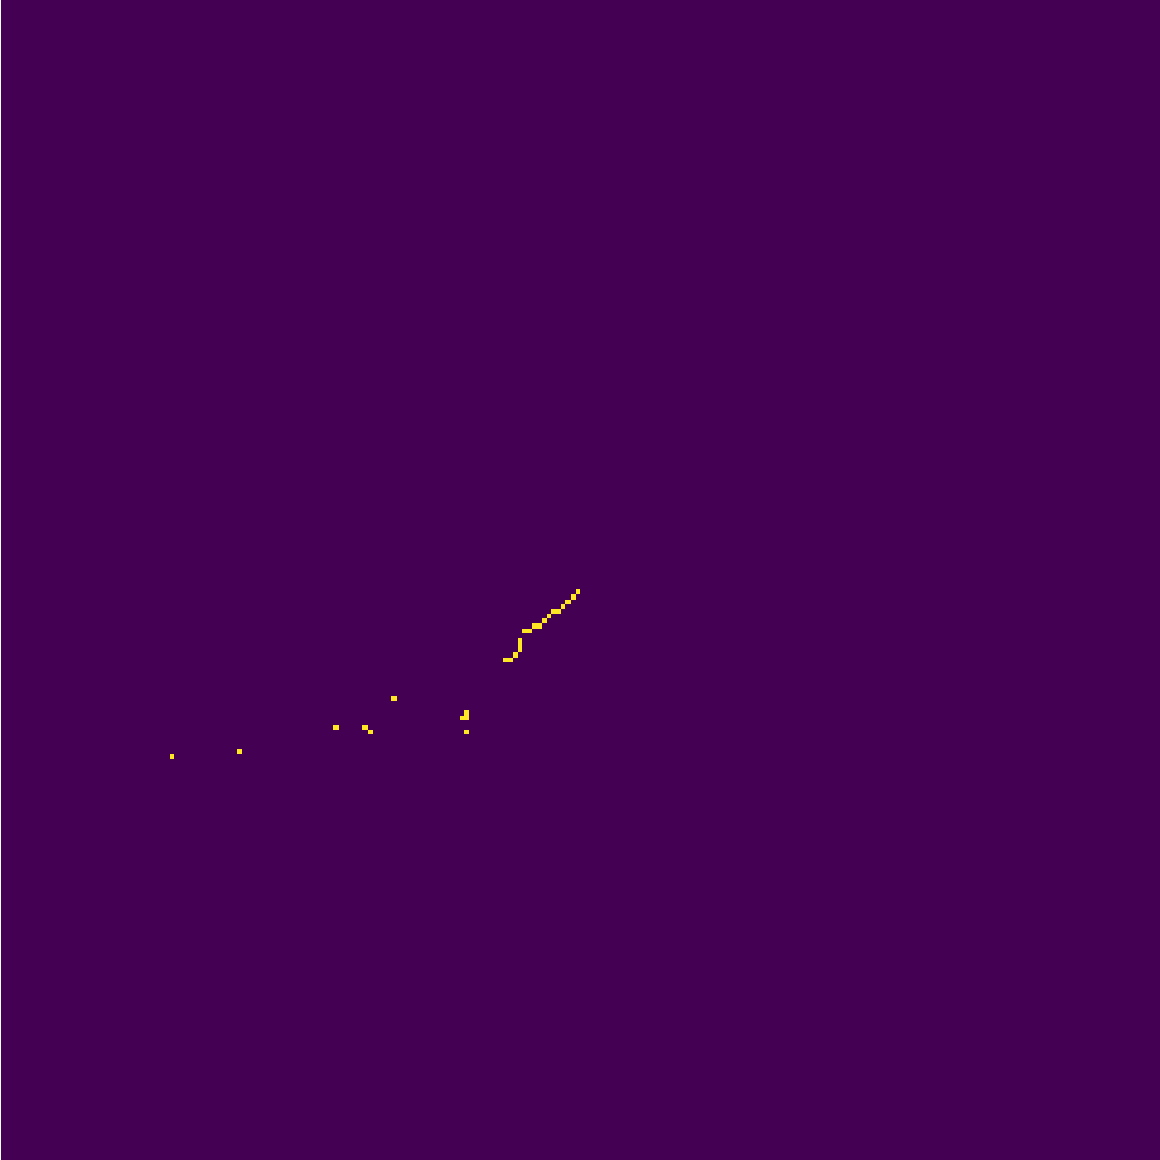
\includegraphics[width=\textwidth]{figures/unet_example_true.pdf}
			\caption {Truth.}
			\label{fig:unet_example_true}
		\end{subfigure} &
		\begin{subfigure}[b]{0.49\textwidth}
			\centering
			\vspace{3mm}
			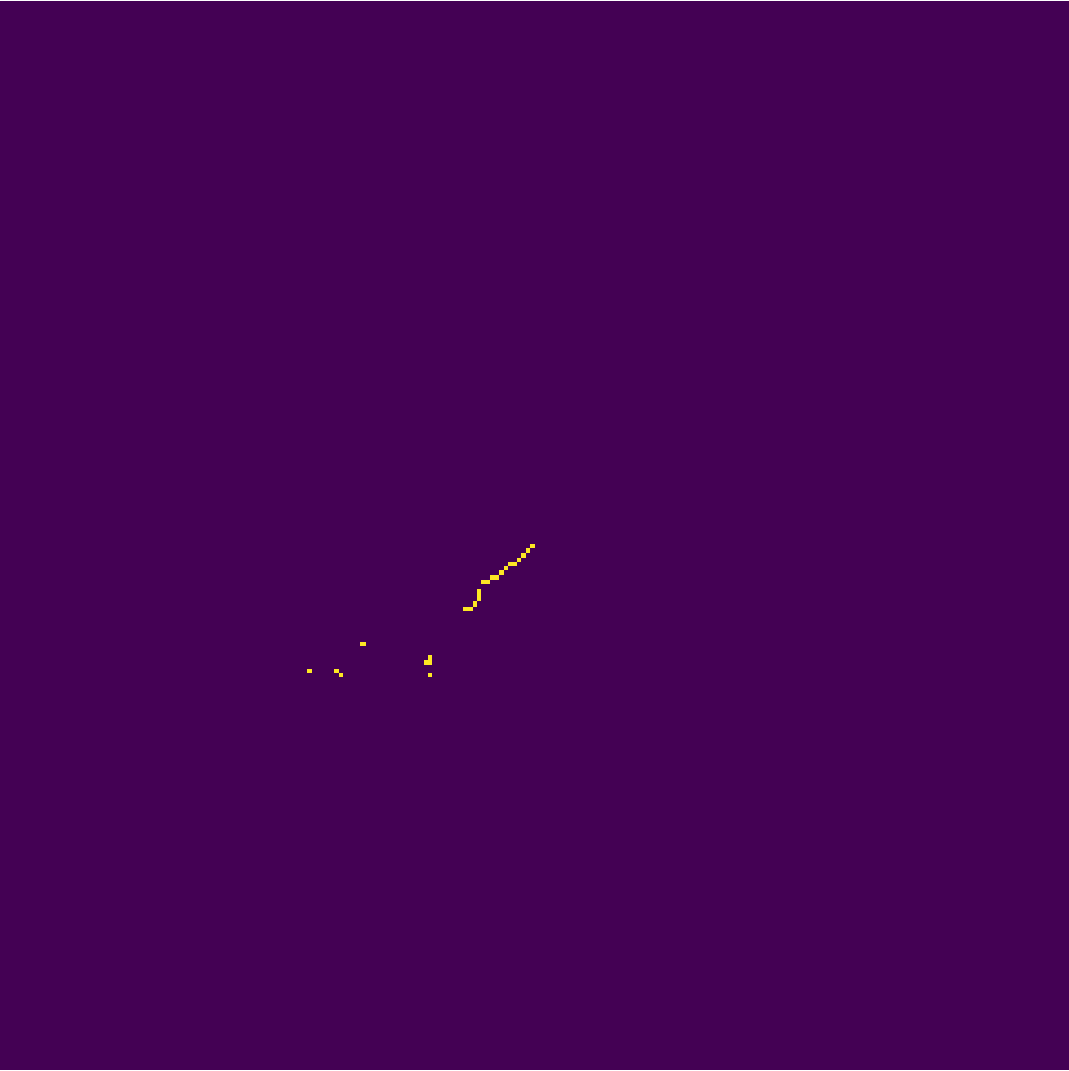
\includegraphics[width=\textwidth]{figures/unet_example_pred.pdf}
			\caption {Output.}
			\label{fig:unet_example_pred}
		\end{subfigure}
	\end{tabularx}

	\caption
	[Example input, truth, and predicted images for U--ResNet.]
	{Example input, truth, and predicted images for U--ResNet.}
	\label{fig:unet_example}
\end{figure}

\subsection{Michel Electron Reconstruction}

An additional dataset was prepared to evaluate the performance of the Michel
electron reconstruction in simulation; this dataset was part of the same batch
of simulation as the training, test, and validation data. For the \protodune{} 
data sample, all data from runs 5387, 5809, and 5770 were used; at the time of 
writing, these runs are the only runs for which the energy calibration 
constants have been calculated.

\subsubsection{Hit Selection}

The U--ResNet produces a sharply peaked output distribution in both data and
simulation, as seen in Figure \ref{fig:unet_pred_data}. The histograms here are
normalised by the number of entries. Both distributions show sharp peaks at zero
and one, but the distribution has slightly sharper peaks in simulation. Hits 
from the input images are selected as Michel electron hits if their score 
exceeds a selection threshold of 0.9. In simulation 7.8\% of hits are 
selected, while in data the fraction selected is 8.0\%. Therefore, there is a 
fractional difference of 2.5\% in the fraction of selected hits between data 
and simulation.  
\begin{figure}
	\centering
	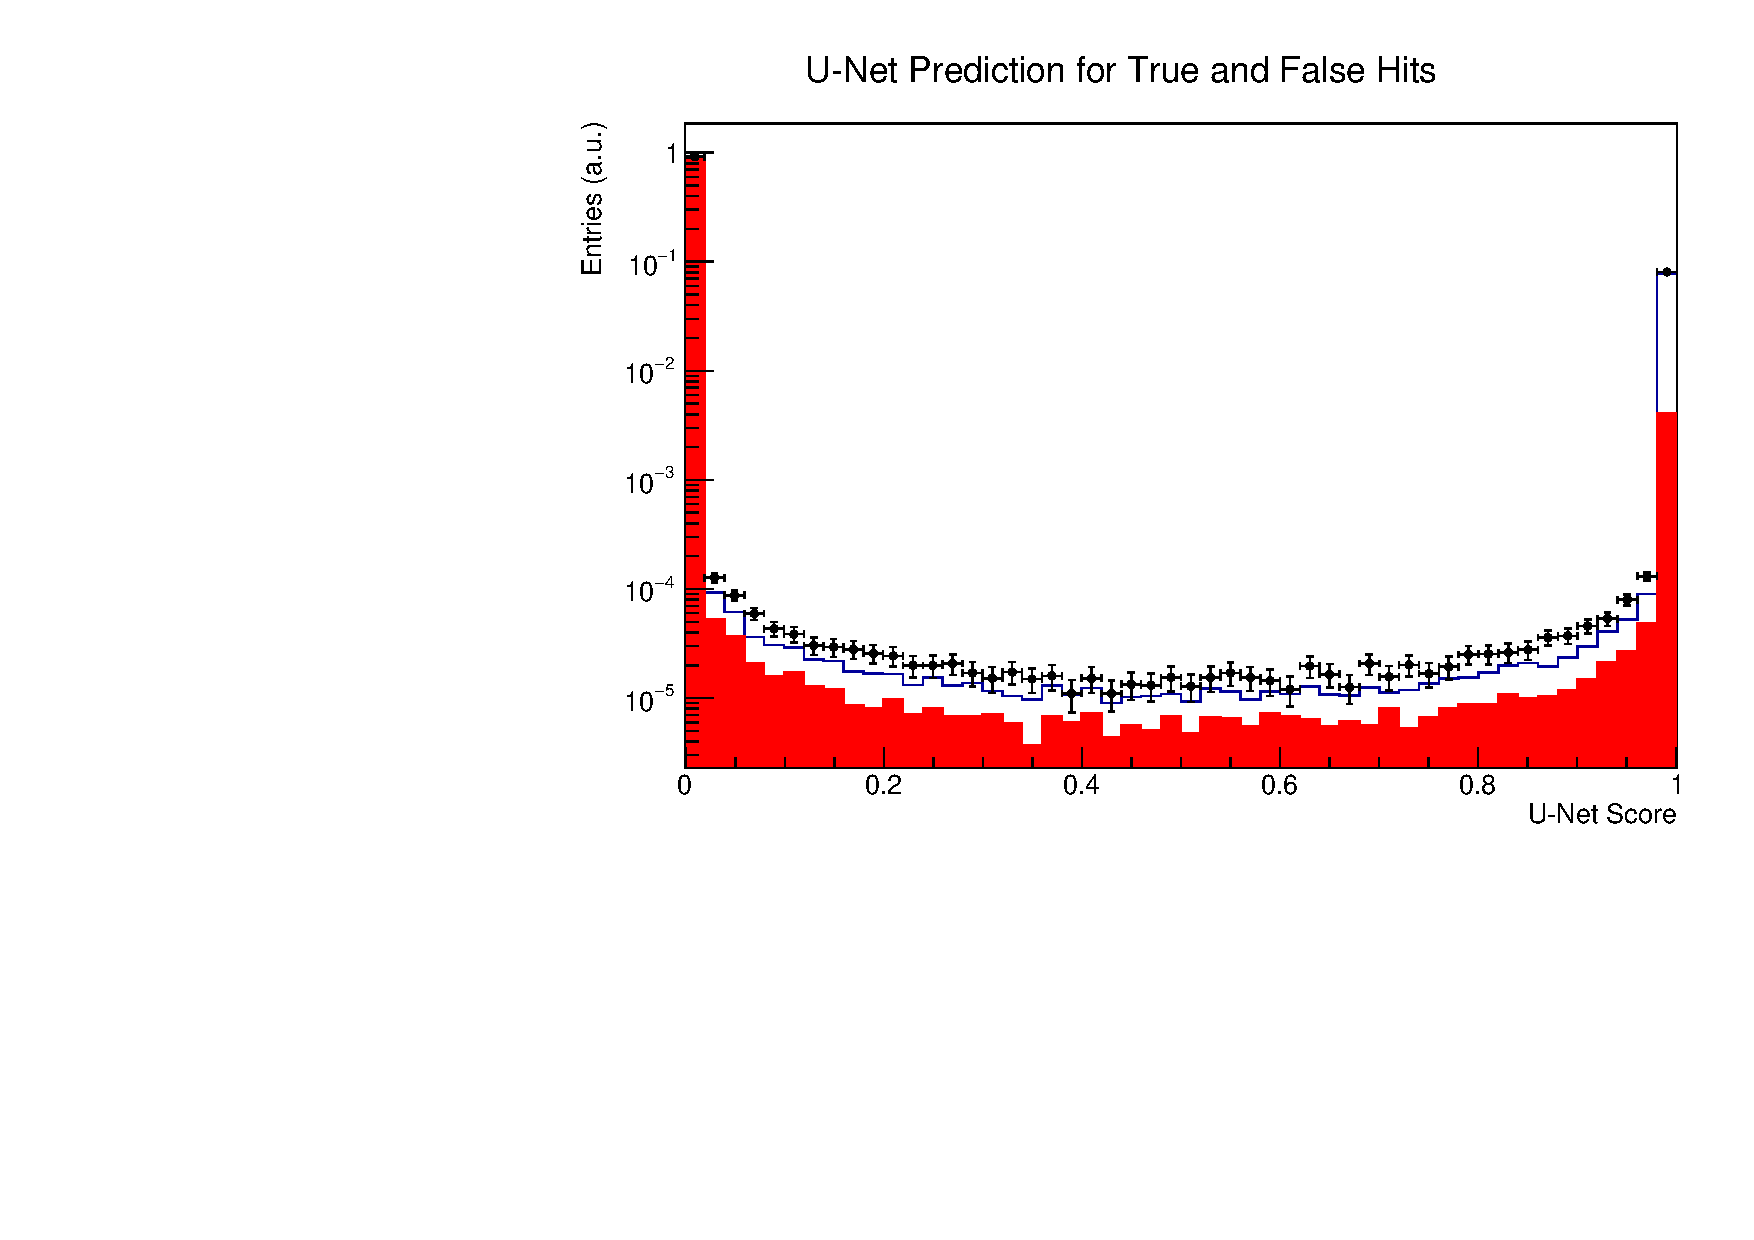
\includegraphics[width=\textwidth]{figures/unet_pred_data.pdf}
	\caption
	[U--ResNet predicted score distribution for hits in Michel electron ionisation
	images.]
	{U--ResNet predicted score distribution for hits in Michel electron
	ionisation images. The simulated results are shown by the red line, with the
	backgrounds, including track hits and hits due to noise, as a shaded red 
	region. The data is shown in black, with statistical error bars. The vertical
	blue line represent the selection cut for hits which were included in the
	energy reconstruction, all hits with a score above 0.9 where included in the
	energy reconstruction.}
	\label{fig:unet_pred_data}
\end{figure}

The performance of the hit tagging algorithm was analysed with the simulated
sample. Based on the score distributions for true and false hits, the purity
and efficiency of the hit tagging algorithm can be evaluated. The purity and 
efficiency are defined as
\begin{align*}
	\mbox{Purity} \quad &= \quad  \frac{N_{TP}}{N_{TP} + N_{FP}} \\
	\vspace{2mm}
	\mbox{Efficiency} \quad &= \quad \frac{N_{TP}}{N_{TP} + N_{FN}}
\end{align*}
where $N_{TP}$, $N_{FP}$, and $N_{FN}$ are the number of true--positives,
false--positives, and false--negatives respectively. These parameters give a
quantitative evaluation of the performance of the hit tagging algorithm.

The purity and efficiency of the hit tagging was calculated for selection 
thresholds in the range $[10^{-7}, 1 - 10^{-7}]$, which returned purities in 
the range 0.91--0.93, and efficiency in the range 0.94--0.96. For thresholds 
outside of this range the purity and efficiency remained constant, except 
for at thresholds of 0 and 1, this is due to the underlying precision in 
Keras, which sets the smallest non--zero float to be $10^{-7}$. The hit tagging 
algorithm produces a high purity and efficiency throughout the range of 
thresholds, however, the combination of the steep score distribution with the 
underlying precision in Keras means that little can be done to optimise the 
performance by varying the threshold in this case.

The number of hits selected per event for data and simulation is shown in
Figure \ref{fig:mich_n_hits}. Around 10 hits are selected on average per 
event, with a tail extending up to around 30 hits. The distribution of the 
backgrounds peaks at a lower energy than the true events, but is only a small
contribution to the overall distribution. A good agreement is seen between the 
data and simulation for the number of selected hits; these hits are then used 
to reconstruct the deposited ionisation energy of the Michel electron.
\begin{figure}
	\centering
	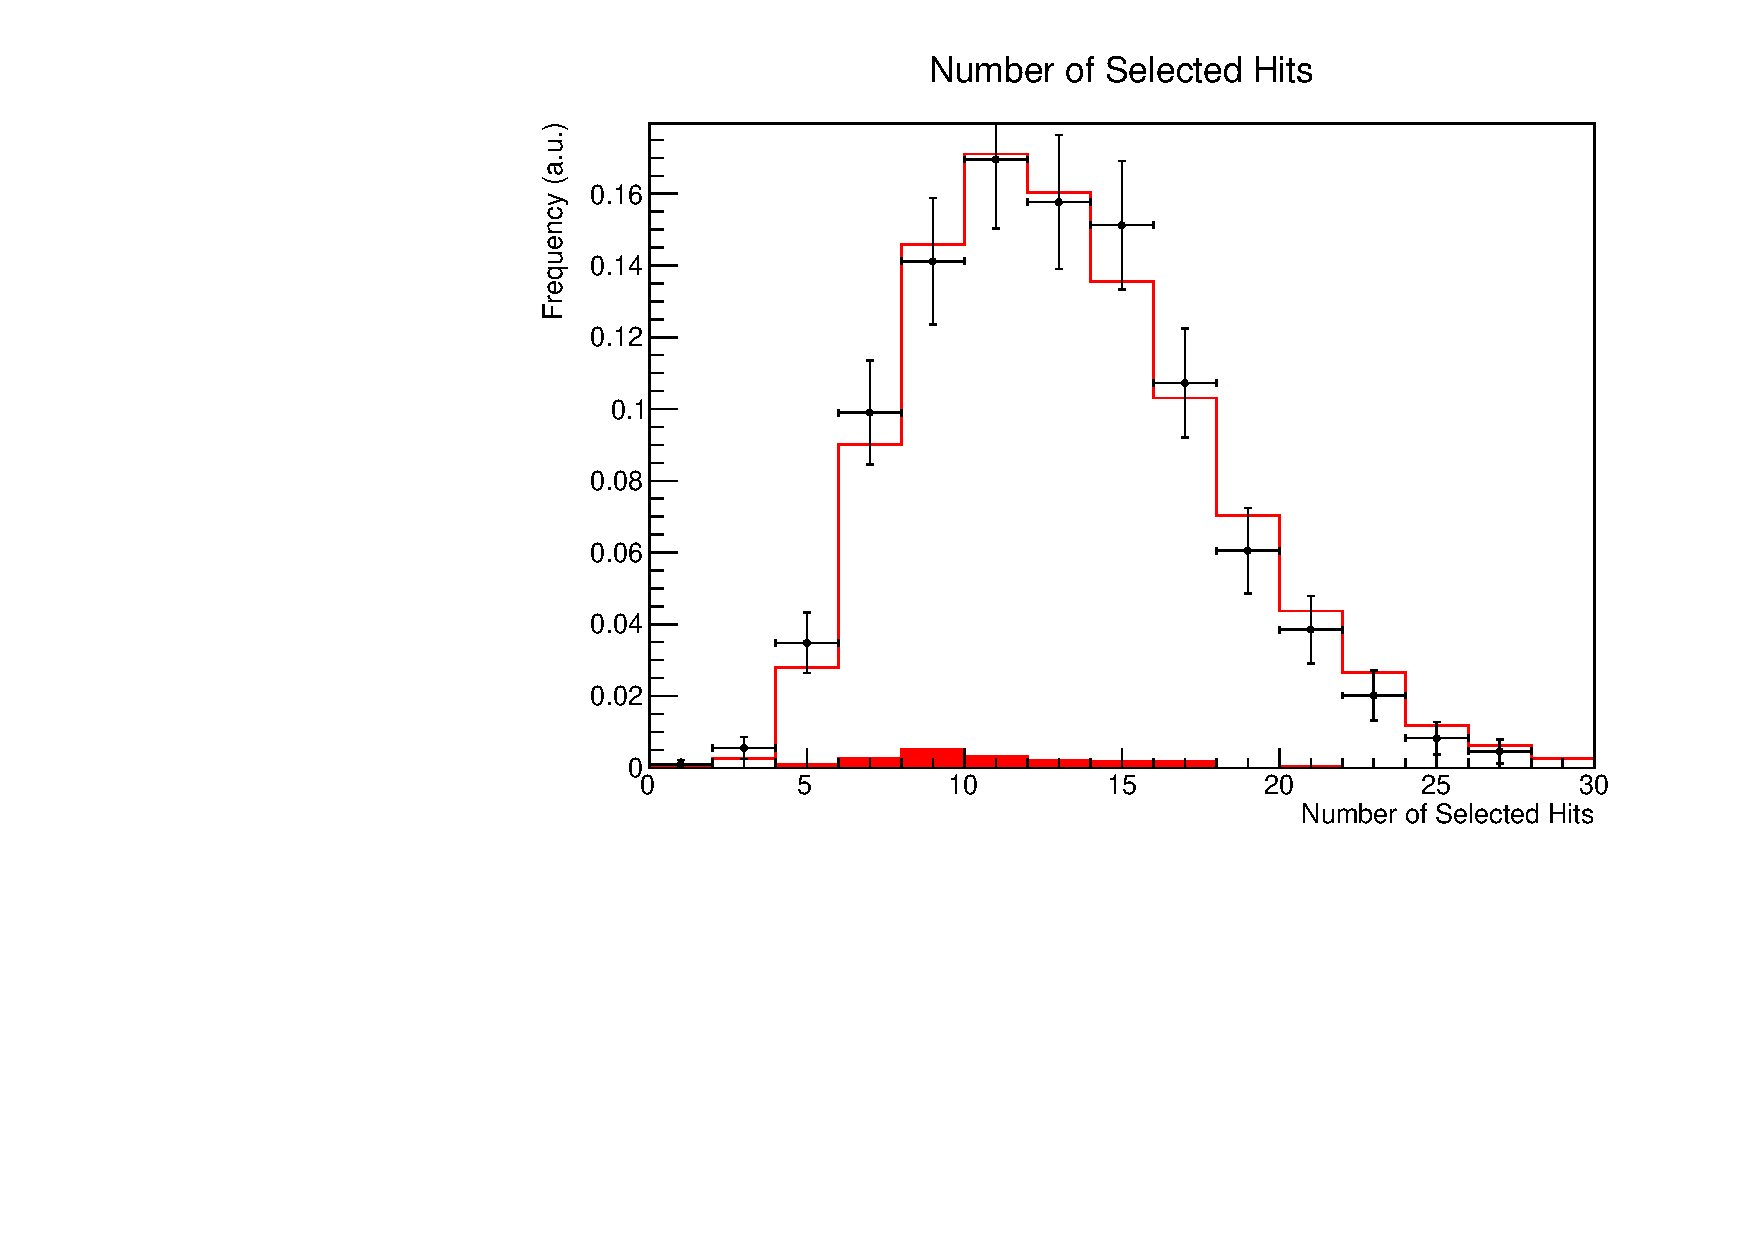
\includegraphics[width=\textwidth]{figures/mich_n_hits.pdf}
	\caption
	[Number of selected hits in reconstructed Michel electron events.]
	{Number of hits selected by the U--ResNet for Michel electron candidate
	events in data and simulation. The distribution in data includes statistical
	error bars.}
	\label{fig:mich_n_hits}
\end{figure}

\subsubsection{Ionisation Energy Reconstruction}

The total ionisation energy is reconstructed by summing the hit--by--hit
ionisation energy for hits selected by the U--ResNet. The ionisation energy for
each hit is reconstructed from the hit integral in ADC as
\begin{equation*}
	E_{hit} = \frac{I_{hit} \times C_X \times C_{YZ} \times N \times W_{ion}}{C \times R}\mbox{,}
\end{equation*}
where $E_{hit}$ is the reconstructed hit energy in MeV, $I_{hit}$ is the
integrated hit charge in ADC, $C_X$ is the X--correction factor which is
dependent on the X (drift) coordinate of the hit within the TPC, $C_{YZ}$ is the
YZ--correction factor which is dependent on the Y (vertical) and Z (beam) 
coordinates of the hit within the TPC, $N$ is a dimensionless normalisation 
factor which normalises the data and MC distributions to give the same 
magnitude, $W_{ion}$ is the ionisation energy of argon in MeV per electron, 
$C$ is a constant conversion factor which has units ADC per electron, and $R$ 
is the recombination factor. The distribution of reconstructed hit energies in 
\protodune{} data and simulation is shown in Figure \ref{fig:hit_ion_reco}, 
which shows a good agreement between data and simulation.

The position dependent calibration matrices correct for any non-uniformity in 
the detector response across the TPC. In the X direction, which is parallel to 
the drift direction, the main contributing factors are attenuation due to 
electron absorption, and variations in the electron drift velocity due to 
space charge effects. The main contributing factor for the YZ--correction 
factor is wire--to--wire response variations.

As discussed in Chapter \ref{ch:energyloss}, the recombination factor is a
$dQ/dx$ dependent factor, which depends on the conditions in the liquid
argon. Due to the shortness of Michel electron tracks and the other charge
deposits, it is challenging to assign $dQ/dx$ on a hit--by--hit basis for this
sample. Therefore, an average recombination factor is used for all hits. The
recombination factor was calculated using the box model\cite{Acciarri2013a}
under \protodune{} operating conditions, which gives an average value of 0.69.

As a result of the spatially dependent calibration factors, the energy of hits
can only be accurately reconstructed for events with a reconstructed true
time, which means that the track needs to have been stitched by the track
stitching algorithm described in Section \ref{sec:reconstruction}. This 
algorithm has a low efficiency due to the fact that only cathode crossing 
tracks can be used, and has a different efficiency in data and simulation due 
to differences in the alignment properties of track segments. The overall 
efficiency of the track stitching algorithm is around 15\% in simulation, and 
only 4\% in data.

\begin{figure}
	\centering
	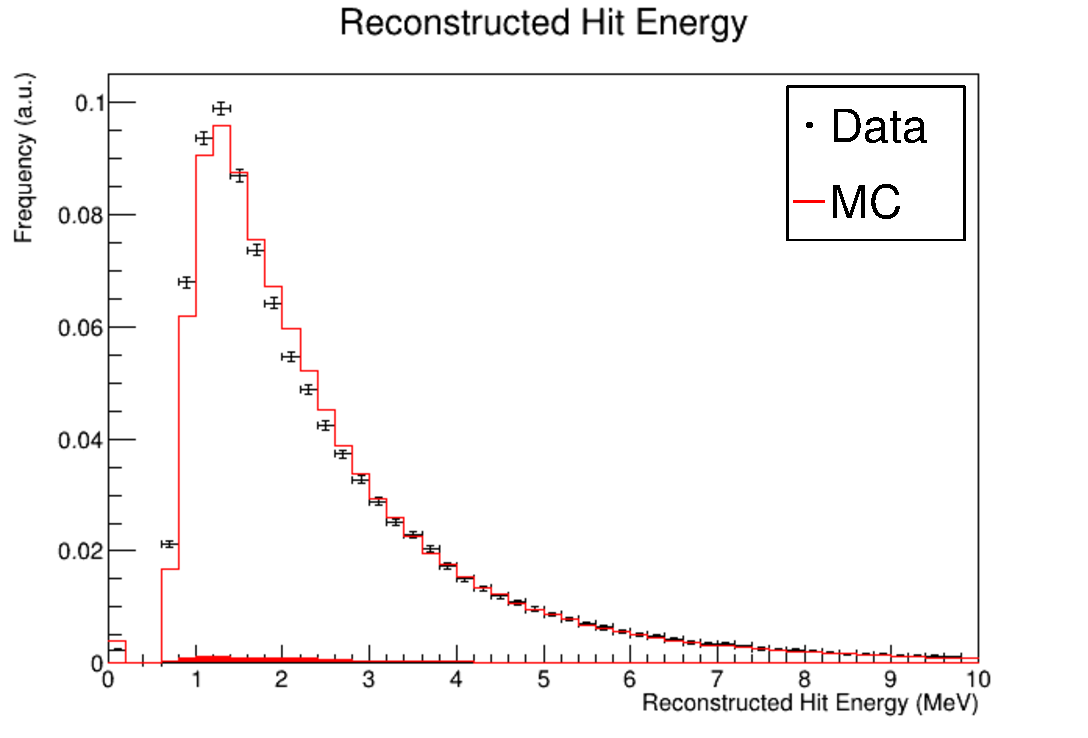
\includegraphics[width=\textwidth]{figures/hit_ion_reco.pdf}
	\caption
	[Reconstructed ionisation energy for hits in U--ResNet input images.]
	{Reconstructed ionisation energy for hits in U--ResNet input images
	in data and simulation. The distribution in data includes statistical error
	bars.}
	\label{fig:hit_ion_reco}
\end{figure}

The reconstructed Michel electron energy is the sum of the reconstructed
ionisation energy for all selected Michel electron hits. The reconstructed
ionisation energy spectrum for Michel electrons in \protodune{} is shown in
Figure \ref{fig:michel_ion_reco}. The distribution peaks at around 20 MeV and
has a tail up to just under 50 MeV, which is consistent with the true
ionisation energy deposited by Michel electrons within a 40 cm radius, shown
in Figure \ref{fig:40_v_80}. Overall, there is a good agreement between the data
and simulation in terms of reconstructed energy. The main difference between the
data and simulation is a slightly longer tail at high energy in data.
\begin{figure}
	\centering
	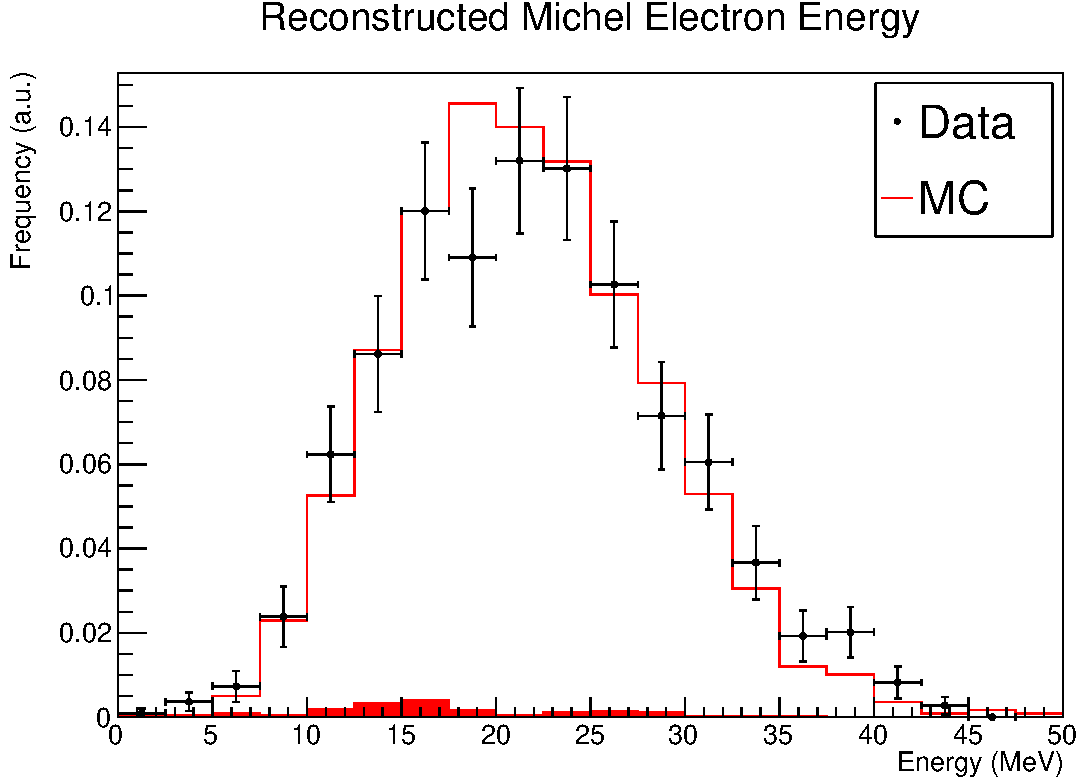
\includegraphics[width=\textwidth]{figures/michel_ion_reco.pdf}
	\caption
	[Reconstructed ionisation energy for Michel electron candidates in
	\protodune{} data and simulation.]
	{ Reconstructed ionisation energy for Michel electron candidates in
	\protodune{} data and simulation. The distribution in data includes
	statistical error bars. }
	\label{fig:michel_ion_reco}
\end{figure}

The performance of the ionisation energy reconstruction was evaluated with the
simulated Michel electron sample. First, the reconstructed ionisation energy was
compared to the true ionisation energy, and a linear scaling factor was
calculated to correct for any energy offset. The correction factor was
calculated based on a linear fit to the distribution of reconstructed energy
against true energy, which is shown in Figure \ref{fig:reco_v_ion}. The
reconstructed energy was corrected based on this linear fit through the origin,
\begin{equation*}
	E_{corr} = E_{reco} \; / \; 0.9823,
\end{equation*}
and the corrected energy was used to estimate the energy resolution and bias of
the Michel electron energy reconstruction.
\begin{figure}
	\centering
	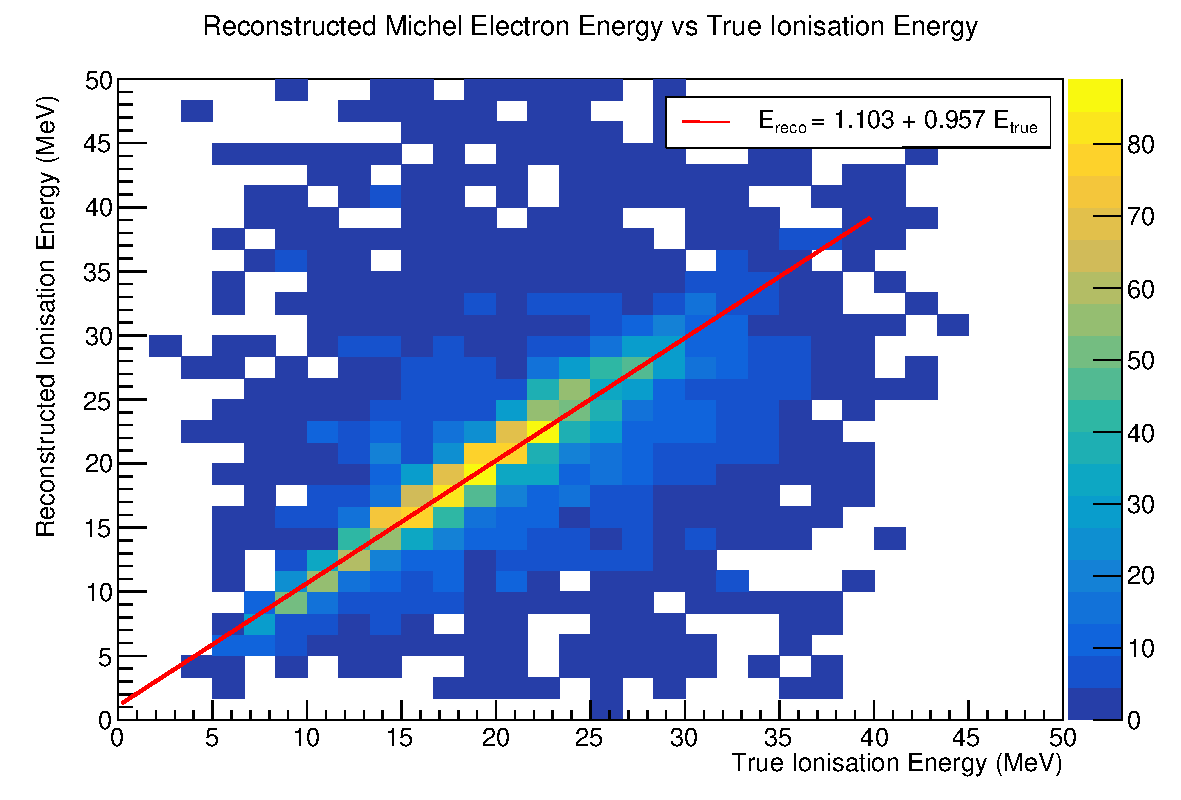
\includegraphics[width=\textwidth]{figures/reco_v_true_ion.pdf}
	\caption
	[Reconstructed ionisation energy vs total deposited ionisation energy for
	Michel electron events in \protodune{} simulation.]
	{ Reconstructed ionisation energy vs total deposited ionisation energy for
	Michel electron events in \protodune{} simulation. }
	\label{fig:reco_v_ion}
\end{figure}

To estimate the resolution and bias of the ionisation energy reconstruction, the
fractional difference between the reconstructed and true ionisation energy was
considered. The fractional difference is defined as,
\begin{equation*}
	\mbox{Fractional Difference} = \frac{E_{corr} - E_{true}}{E_{true}},
\end{equation*}
such that the spread of the distribution is a measure of the fractional
uncertainty of the reconstructed energy. The energy resolution and bias were
estimated by fitting a gaussian to the fractional difference distribution; the
standard deviation of the gaussian was taken to be an estimate of the energy
resolution, and the mean as an estimate of the bias. The distribution of the 
fractional difference for all events, and the associated gaussian fit, are 
shown in Figure \ref{fig:frac_diff_ion}. Based on this fit the energy 
resolution was estimated to be around 10\% and the bias around 1\%. However, 
it is worth noting that the fractional difference distribution has a fairly 
significant tail for negative fractional differences and, therefore, the fit 
was restricted to the central region of the distribution.
\begin{figure}
	\centering
	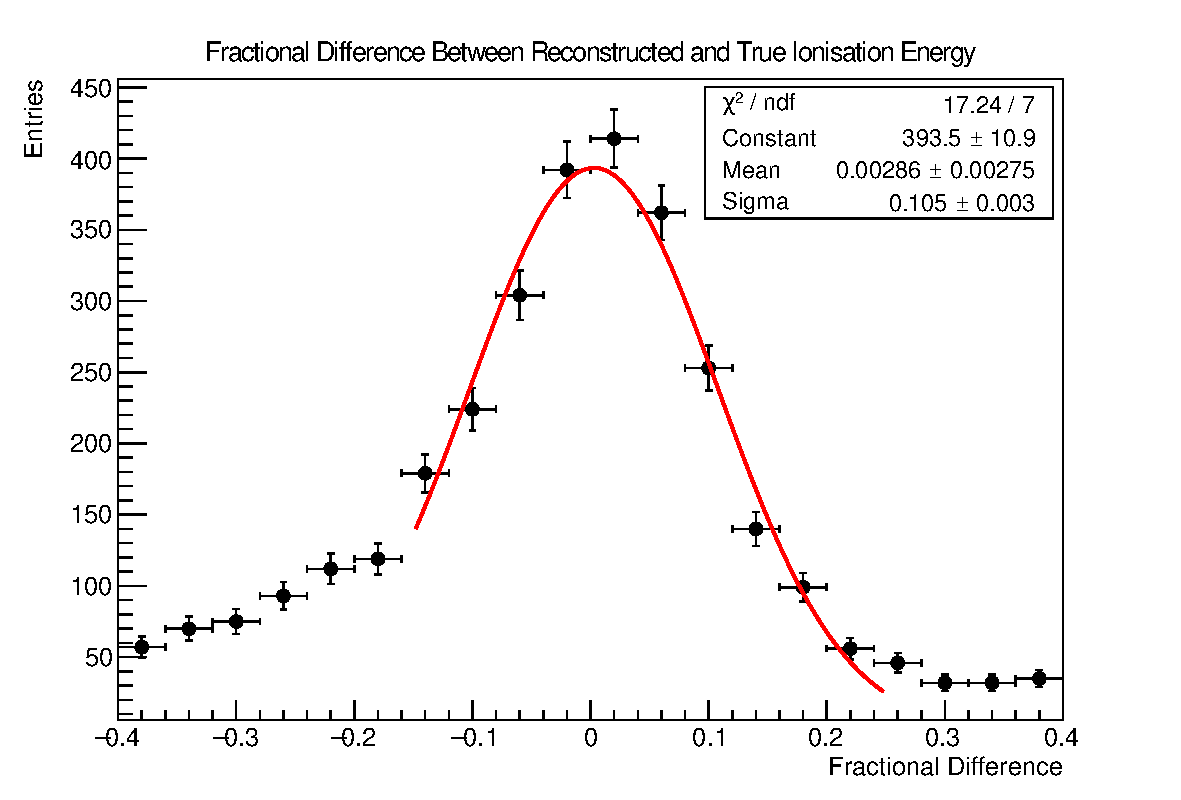
\includegraphics[width=\textwidth]{figures/frac_diff_ion.pdf}
	\caption
	[Fractional energy difference between reconstructed and true Michel electron
	energy.]
	{Fractional energy difference between reconstructed and true Michel electron
	ionisation energy in \protodune{} simulation, with statistical error bars.}
	\label{fig:frac_diff_ion}
\end{figure}

Studies into the energy resolution and bias as a function of energy gave
insights into the source of the tail in Figure \ref{fig:frac_diff_ion}. These
were investigated by binning the fractional energy difference distribution in
terms of true ionisation energy, and performing the same gaussian fit to the
fractional difference distribution for each energy bin. The measured energy
resolution and bias as a function of true ionisation energy are shown in
Figure \ref{fig:res_and_bias_ion}, the associated fits are given in Appendix
\ref{ch:energyfits}.
\begin{figure}
	\centering
	\begin{subfigure}[b]{\textwidth}
		\centering
		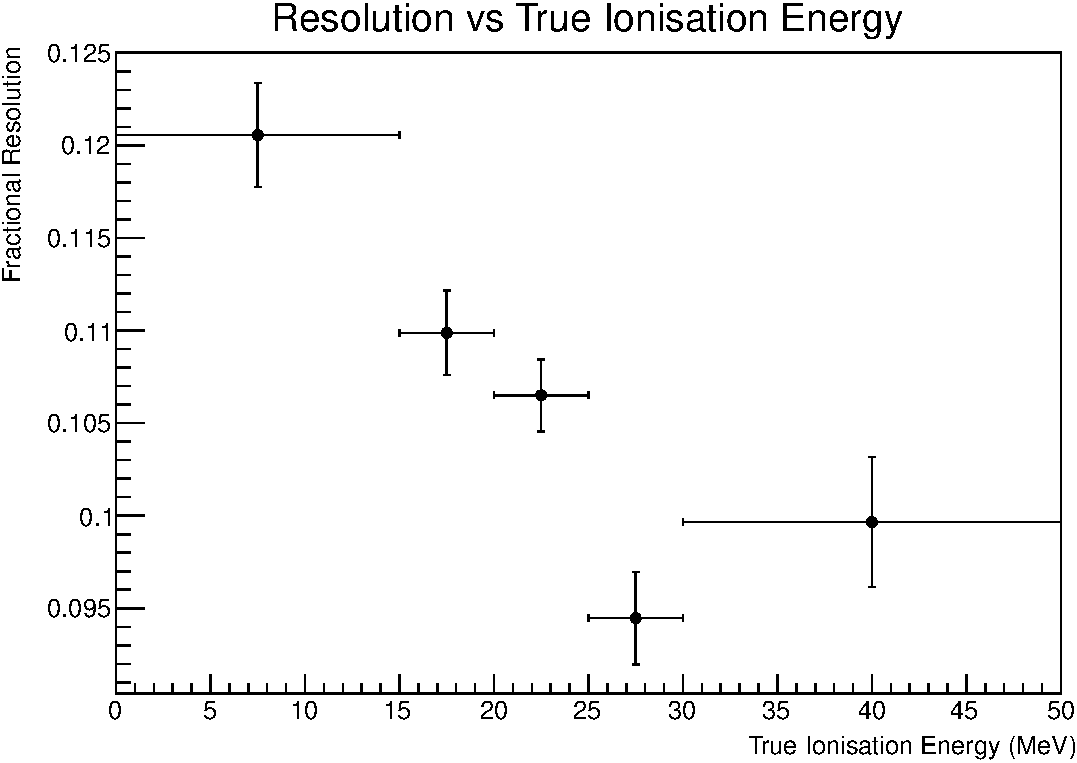
\includegraphics[width=0.95\textwidth]{figures/res_v_energy_ion.pdf}
		\caption {Resolution.}
		\label{fig:res_ion}
	\end{subfigure}
	\begin{subfigure}[b]{\textwidth}
		\centering
		\vspace{5mm}
		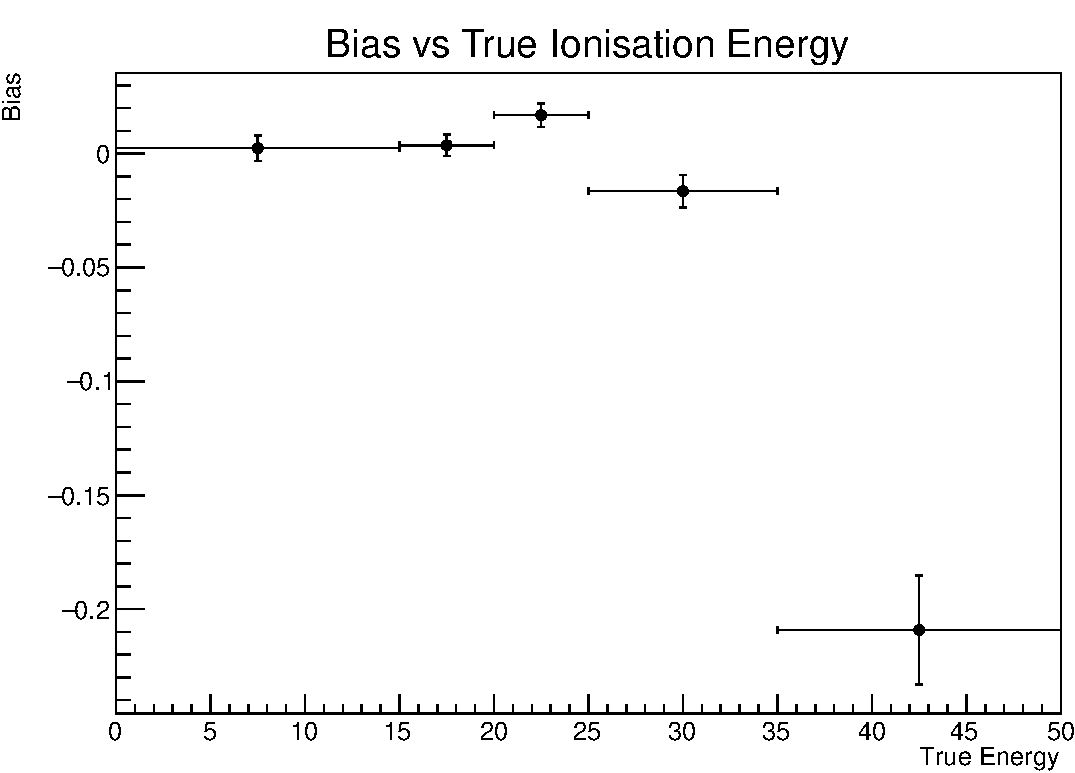
\includegraphics[width=0.95\textwidth]{figures/bias_v_energy_ion.pdf}
		\caption {Bias.}
		\label{fig:bias_ion}
	\end{subfigure}
	\caption
	[Energy resolution and bias for Michel electrons as a function of true
	ionisation energy deposition.]
	{Energy resolution and bias for Michel electrons as a function of true
	ionisation energy deposition in \protodune{} simulation. The error bars
	represent the statistical uncertainty only.}
	\label{fig:res_and_bias_ion}
\end{figure}

The energy resolution and bias as a function of energy demonstrate that the
energy reconstruction algorithm is capable of good energy reconstruction
performance. However, it is important to note that above around 25 MeV there is
significant tail for negative fractional differences. This is due to a reduction
in the hit tagging efficiency in the high energy region, which causes less of
the initial Michel electron energy to be collected by the CNN. No attempt was
made to fit this tail and, therefore, the estimated energy resolution and bias
based on the gaussian fits overstate the performance in the high energy region.
A more conservative estimate can be made by considering the mean and RMS of the
distribution. Table \ref{tab:gaus_v_mean} gives a comparison between the
estimated bias and resolution based on these two methods.
\begin{table}
	\centering
	\bgroup
	\def\arraystretch{1.5}
	\begin{tabular}{c|c|c|c|c}
		Energy Bin & Gaussian Mean (\%) & Gaussian Sigma (\%) & Mean  (\%)     & RMS (\%)   \\ \hline
		0--15 MeV  & $+0.3 \pm 0.3$     & $12.1 \pm 0.3$      & $+0.8 \pm 0.2$ & $15.0 \pm 0.2$  \\
		15--20 MeV & $+1.8 \pm 0.2$     & $11.0 \pm 0.2$      & $+1.8 \pm 0.2$ & $14.7 \pm 0.2$ \\
		20--25 MeV & $+0.9 \pm 0.1$     & $10.6 \pm 0.2$      & $+0.0 \pm 0.2$ & $14.5 \pm 0.1$ \\
		25--30 MeV & $-0.1 \pm 0.2$     & $9.5 \pm 0.2$       & $-3.4 \pm 0.2$ & $14.9 \pm 0.2$ \\
		30--50 MeV & $-2.9 \pm 0.4$     & $10.0 \pm 0.4$      & $-8.6 \pm 0.3$ & $16.0 \pm 0.2$\\

	% 0 0.00815335 0.00267316 0.150079 0.00189021
	% 15 0.0175661 0.00222734 0.14724 0.00157496
	% 20 3.92331e-05 0.00203149 0.145149 0.00143648
	% 25 -0.0338276 0.00227804 0.148458 0.00161082
	% 30 -0.0859376 0.00251298 0.16026 0.00177694

	\end{tabular}
	\egroup
	\caption
	[Comparison of energy resolution estimates for Michel electron ionisation
	energy.]
	{ Comparison of energy resolution estimates for Michel electron ionisation
	energy from \protodune{} simulation. }
	\label{tab:gaus_v_mean}
\end{table}

\subsubsection*{Contributions to Ionisation Energy Resolution}
The ionisation energy resolution is made up of a combination of the hit--by--hit
energy resolution, and the spread introduced due to imperfect hit tagging. The
contribution from the hit--by--hit energy resolution can be estimated by
considering the fractional energy difference in the case of perfect hit tagging,
which sums the reconstructed energy of all the true Michel electron hits in
the image. The sum over the hits in each image is considered because this
allows the error in the hit--by--hit recombination factor, which arises due to
the use of an average recombination factor during reconstruction, to be
averaged over the hits in the image. The fractional energy difference in this
case is fit with a gaussian distribution, which is shown in Figure
\ref{fig:michel_hit_res}.
\begin{figure}
	\centering
	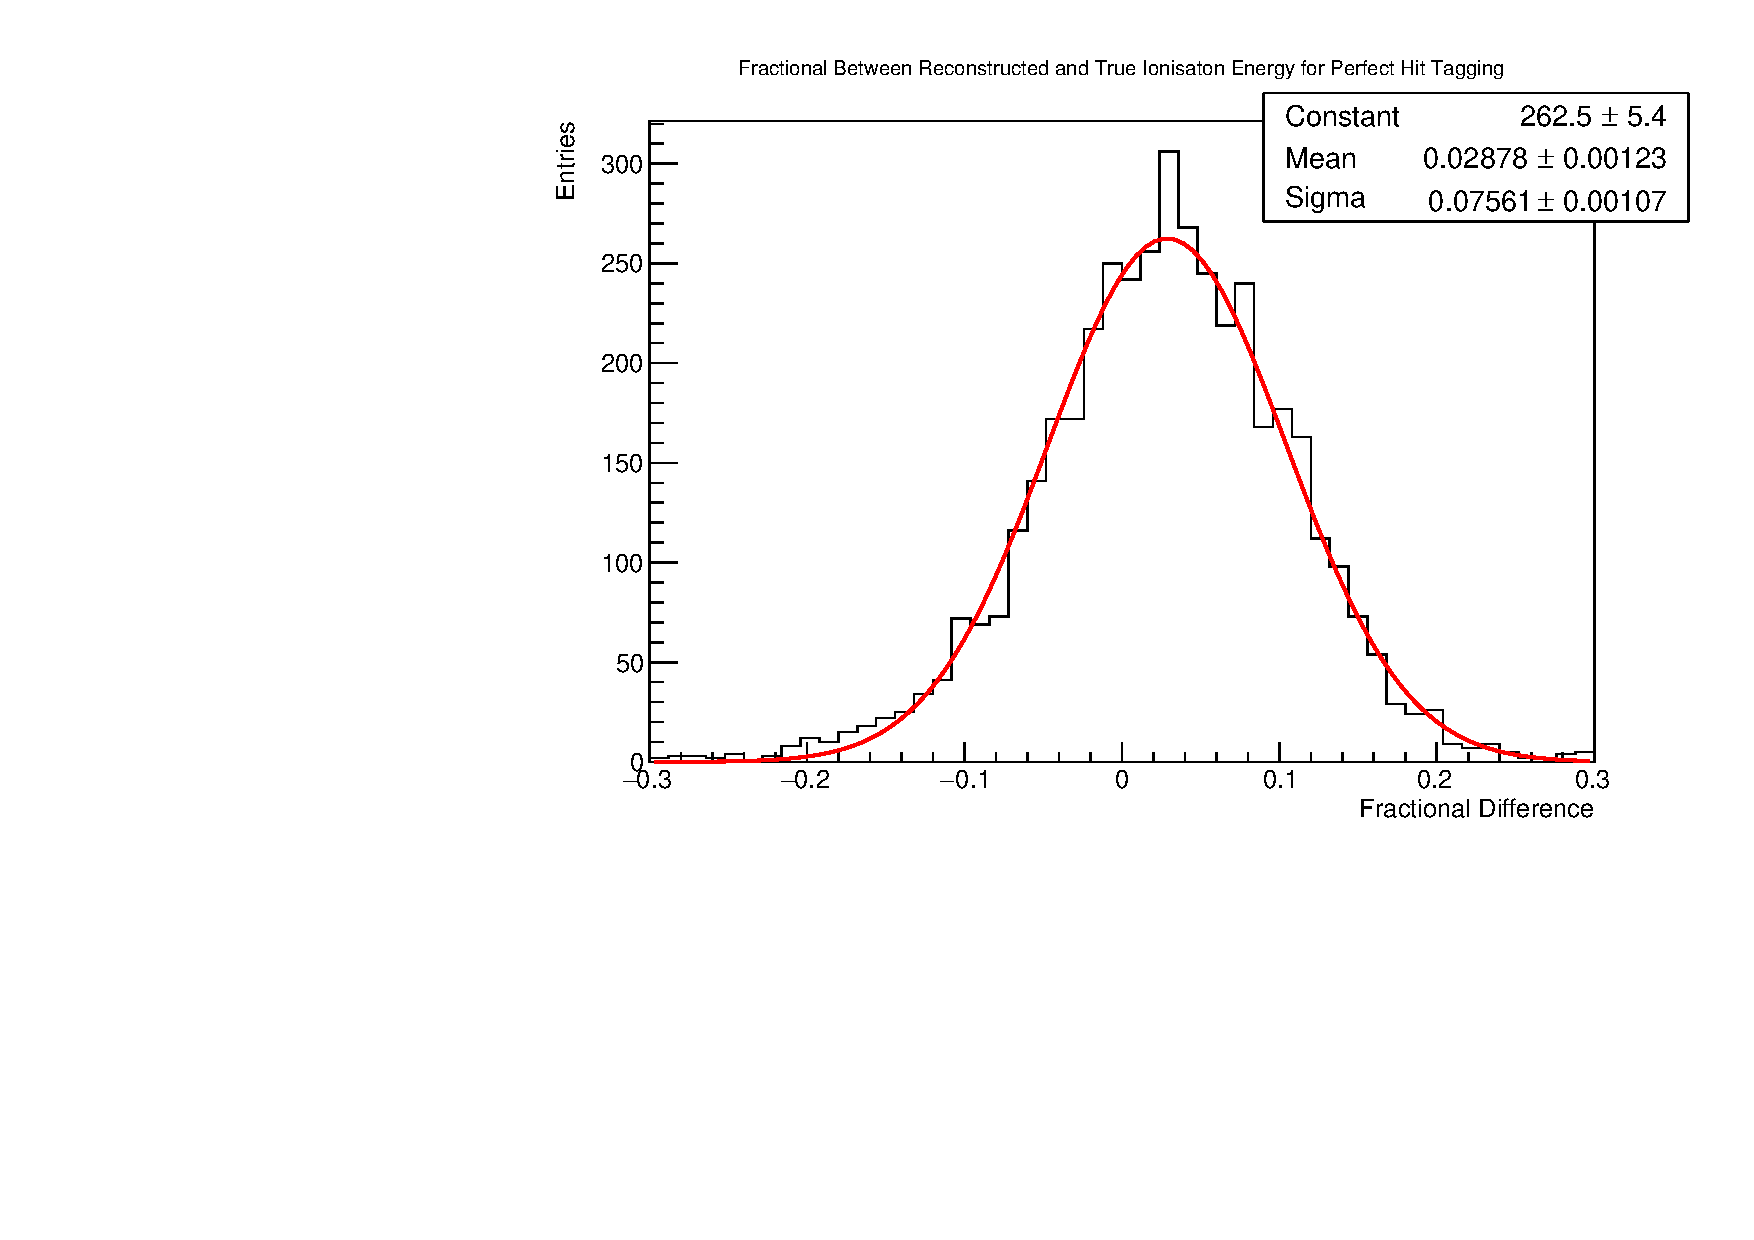
\includegraphics[width=\textwidth]{figures/michel_hit_energy_resolution.pdf}
	\caption
	[Energy uncertainty contribution from hit energy reconstruction for Michel
	electron ionisation energy reconstruction.]
	{The fractional difference between the true ionisation energy deposition and
	the reconstructed ionisation energy deposition for Michel electron
	reconstructed with perfect hit tagging, with statistical error bars. The
	distribution is fit with a gaussian, which is shown in red, and the fit
	parameters are shown in the top right corner.}
	\label{fig:michel_hit_res}
\end{figure}

The contribution to the ionisation energy resolution due to the hit energy
reconstruction was estimated based on the parameters from the gaussian fit in
Figure \ref{fig:michel_hit_res}. The bias in the hit energy reconstruction was
estimated to be around 3\%, and the resolution was estimated to be
approximately 8\%. The remaining energy resolution and bias seen in the Michel
electron ionisation energy reconstruction is a result of the spread due to
imperfect hit tagging.

\subsubsection*{Comparison to Other LArTPC Experiments} \label{ME_COMP}

In order to put the performance of the Michel electron energy
reconstruction into context, it is useful to compare the results presented
here with those from other LArTPC experiments. The comparisons here are
restricted to the 0--30 MeV region, recognising that improvements are still 
required in order to reduce the tail for higher ionisation energies. The closest
comparison is against the MicroBooNE experiment, which is a surface level LArTPC
that used ionisation energy for the reconstruction\cite{Acciarri:2017sjy}. 
LArIAT and ICARUS have also performed Michel electron 
reconstruction\cite{Amoruso:2003sw,Foreman_2016}, however, LArIAT used the 
scintillation light for reconstruction, and ICARUS is deep underground and, 
therefore, has significantly less backgrounds.

The MicroBooNE experiment gives the closest comparison for Michel electron
reconstruction, as both MicroBooNE and \protodune{} are surface level TPCs, and
they both use ionisation energy for Michel electron reconstruction. In
MicroBooNE, the ionisation energy resolution for Michel electrons was found to
be between 15--25\% in the 0--30 MeV region\cite{Acciarri:2017sjy}. In this 
region the algorithm developed here gives an improved energy resolution of 
around 10--12\%, which highlights the potential of the semantic segmentation 
approach if the bias at higher energies can be improved such that the approach
is applicable across the full energy range.

ICARUS also used ionisation energy for Michel electron reconstruction, however,
the ICARUS detector was located deep underground and, therefore, they were
subject to much lower backgrounds. In ICARUS, the ionisation energy resolution
was measured to be in the range of 3--8\%\cite{Amoruso:2003sw}, however, these
results did not take into account any radiated energy deposits, which form an
important part of the Michel electron signature. Therefore, the results from
ICARUS are not directly comparable to the measured energy resolution presented
here.

LArIAT is a significantly smaller TPC than \protodune{} and, therefore, despite
being at surface level, there is a sufficiently low rate of cosmic--rays that the
photon detection system could be used to tag and measure Michel electron events.
LArIAT measured an energy resolution on the order of 20\% for Michel electrons
based on the scintillation light signal\cite{Foreman_2016}.

In DUNE, both the ionisation energy and scintillation light will be used to
reconstruct supernova neutrinos. The results in the DUNE technical design
report are based on energy resolution estimates from the standard
LArSoft reconstruction framework, which give an ionisation energy resolution of
around 20\%, and a scintillation light energy resolution in the range of
10-20\%\cite{Abi:2020evt}. Therefore, if the tail at high energy can be
improved, a semantic segmentation algorithm, similar to the one presented
here, may be able to improve the energy reconstruction performance for
supernova neutrinos in the DUNE Far Detector. This is an important factor in
many supernova neutrino physics studies, in which the mean neutrino energy is an
important parameter\cite{Abi:2020evt}.

\section{Conclusion} \label{ME_EU}

In the energy regime of Michel electrons, and supernova neutrinos, the
electromagnetic energy deposition of electrons moves from an 
ionisation--dominated to a radiation--dominated region. As such, these events 
have a signature, which contains both track--like and a shower--like 
components and. Therefore, they require a unique reconstruction algorithm in 
order to maximise the energy collected from the events.

This chapter has presented a novel Michel electron reconstruction algorithm 
based on machine learning techniques. A sample of Michel electrons was 
selected in \protodune{} data with a purity of over 98\% and an overall 
efficiency of around 6\%. The low efficiency is acceptable due to the very high
rate of Michel electron events in \protodune{}, which will lead to a large high
purity sample once more calibrated data has been collected and processed. The 
ionisation energy of these events was reconstructed based on a semantic 
segmentation algorithm, which uses a U--ResNet CNN architecture. The 
performance of this algorithm shows an improvement in energy resolution over 
similar experiments, with an ionisation energy resolution of around 10-15\%.  
However, there is still need for improvement, particularly in the high energy 
region where a large tail is seen in the fractional difference distribution.

The promising results in the low energy region based on this method, suggest
that with further study the semantic segmentation approach could prove to be an
effective algorithm for reconstructing low energy particles in LArTPCs. In 
order to increase the performance in the high energy region, it may be useful 
to consider increasing the amount of training data in this region. At the time 
of writing, there is insufficient \protodune{} simulation to produce a flat 
training sample with sufficient data. Therefore, this remains as a possible 
future study, which has the potential to significantly increase the 
performance of this algorithm, by increasing the generalisability across the 
energy range.

While Michel electrons provide an interesting sample with which to study low
energy electron reconstruction, it is important to note the differences between
Michel electron and supernova neutrino events in LArTPCs, and the
different conditions between \protodune{} and DUNE, when considering the
applicability of these results to supernova neutrino reconstruction in DUNE. A 
number of relevant differences will now be detailed.

Firstly, Michel electron events are accompanied by a muon track in LArTPC 
events, which aids with event selection but also masks some of the Michel 
electron energy due to the presence of the Bragg peak of the muon. Second, the 
peak of the Michel electron energy spectrum is at around 40 MeV as opposed to 
around 15 MeV in the case of supernova neutrinos. As a result, Michel electron 
events contain a larger fraction of radiated energy deposition than supernova 
neutrinos, and as such the energy reconstruction results in the lower energy 
region are likely to give a more representative prediction of the expected 
energy resolution for supernova neutrinos in DUNE. Finally, DUNE will have a 
significantly lower background of cosmic--ray events than \protodune{}, which 
will give two benefits: the hit tagging algorithm will have fewer unnecessary 
hits to filter due to cosmic--ray activity, and it will be significantly 
easier to match signals from the TPC to those in the photon detectors, which 
will allow for both ionisation and scintillation energy deposits to be 
utilised during energy reconstruction.

As a result of these differences, it will be important to conduct separate
studies of supernova neutrino reconstruction under the operating conditions
expected in the DUNE far detector. This study has demonstrated the considerable
promise of a semantic segmentation approach to low energy electron
reconstruction in LArTPCs and it outperforms the current supernova neutrino 
energy resolution estimates based on ionisation energy deposits in the region of
interest for supernova neutrinos. As such this would be an interesting 
approach to consider when studying the capabilities of DUNE when it comes to 
supernova neutrino reconstruction, and may lead to improved energy resolution 
for supernova neutrino reconstruction in DUNE.
